\documentclass[11pt,english,singlespacing,headsepline]{MastersDoctoralThesis}

\usepackage[utf8]{inputenc} % Required for inputting international characters
\usepackage[T1]{fontenc} % Output font encoding for international characters

\usepackage{amsmath}
\usepackage{amsthm}
\usepackage{amssymb}
\usepackage{tikz}
\usepackage{setspace}
\usepackage{extarrows}

\usetikzlibrary{arrows,chains,matrix,positioning,scopes}
\makeatletter
\tikzset{join/.code=\tikzset{after node path={%
\ifx\tikzchainprevious\pgfutil@empty\else(\tikzchainprevious)%
edge[every join]#1(\tikzchaincurrent)\fi}}}
\makeatother

\tikzset{>=stealth',every on chain/.append style={join},
         every join/.style={->}}
\tikzstyle{labeled}=[execute at begin node=$\scriptstyle,
   execute at end node=$]

\newtheorem{defi}{Definition}
\newtheorem{lem}{Lemma}
\newtheorem{conj}{Conjecture}
\newtheorem{rem}{Remark}
\newtheorem{prop}{Proposition}
\newtheorem{thm}{Theorem}
\newtheorem{cor}{Corollary}
\newtheorem{expl}{Example}

\usepackage{mathpazo} % Use the Palatino font by default

%\usepackage[backend=bibtex,style=authoryear,natbib=true]{biblatex} % Use the bibtex backend with the authoryear citation style (which resembles APA)

%\addbibresource{example.bib} % The filename of the bibliography

%\usepackage[autostyle=true]{csquotes} % Required to generate language-dependent quotes in the bibliography

\usepackage[ngerman]{datetime}

\newdateformat{myformat}{\THEDAY{. }\monthnamengerman[\THEMONTH] \THEYEAR}

%----------------------------------------------------------------------------------------
%	MARGIN SETTINGS
%----------------------------------------------------------------------------------------

\geometry{
	paper=a4paper, % Change to letterpaper for US letter
	inner=2.5cm, % Inner margin
	outer=3.8cm, % Outer margin
	bindingoffset=.5cm, % Binding offset
	top=1.5cm, % Top margin
	bottom=1.5cm, % Bottom margin
	%showframe, % Uncomment to show how the type block is set on the page
}

%----------------------------------------------------------------------------------------
%	THESIS INFORMATION
%----------------------------------------------------------------------------------------

\thesistitle{The Cheeger constants of a simplex} % Your thesis title, this is used in the title and abstract, print it elsewhere with \ttitle
\supervisor{Prof. Dr. Dmitry \textsc{Feichtner-Kozlov}} % Your supervisor's name, this is used in the title page, print it elsewhere with \supname
\examiner{} % Your examiner's name, this is not currently used anywhere in the template, print it elsewhere with \examname
\degree{Dr. rer. nat.} % Your degree name, this is used in the title page and abstract, print it elsewhere with \degreename
\author{Kai Michael \textsc{Renken}} % Your name, this is used in the title page and abstract, print it elsewhere with \authorname
\addresses{} % Your address, this is not currently used anywhere in the template, print it elsewhere with \addressname

\subject{Mathematics} % Your subject area, this is not currently used anywhere in the template, print it elsewhere with \subjectname
\keywords{} % Keywords for your thesis, this is not currently used anywhere in the template, print it elsewhere with \keywordnames
\university{\href{http://www.uni-bremen.de}{Universität Bremen}} % Your university's name and URL, this is used in the title page and abstract, print it elsewhere with \univname
\department{\href{http://alta.uni-bremen.de}{ALTA - Institute for Algebra, Geometry, Topology and their applications}} % Your department's name and URL, this is used in the title page and abstract, print it elsewhere with \deptname
\group{{CALTOP}} % Your research group's name and URL, this is used in the title page, print it elsewhere with \groupname
\faculty{\href{http://fb3.uni-bremen.de}{Fachbereich 3 - Mathematik und Informatik}} % Your faculty's name and URL, this is used in the title page and abstract, print it elsewhere with \facname

\AtBeginDocument{
\hypersetup{pdftitle=\ttitle} % Set the PDF's title to your title
\hypersetup{pdfauthor=\authorname} % Set the PDF's author to your name
\hypersetup{pdfkeywords=\keywordnames} % Set the PDF's keywords to your keywords
}

\begin{document}

\frontmatter % Use roman page numbering style (i, ii, iii, iv...) for the pre-content pages

\pagestyle{plain} % Default to the plain heading style until the thesis style is called for the body content

%----------------------------------------------------------------------------------------
%	TITLE PAGE
%----------------------------------------------------------------------------------------

\begin{titlepage}
\begin{center}

\includegraphics[scale=0.3]{Logo.jpg} % University/department logo - uncomment to place it

\textsc{\Large Dissertation}\\[0.5cm] % Thesis type

\HRule \\[0.4cm] % Horizontal line
{\huge \bfseries \ttitle\par}\vspace{0.4cm} % Thesis title
\HRule \\[1.5cm] % Horizontal line
 
\begin{minipage}[t]{0.4\textwidth}
\begin{flushleft} \large
\emph{Autor:}\\
{\authorname} % Author name - remove the \href bracket to remove the link
\end{flushleft}
\end{minipage}
\begin{minipage}[t]{0.4\textwidth}
\begin{flushright} \large
\emph{Betreuer:} \\
{\supname} % Supervisor name - remove the \href bracket to remove the link  
\end{flushright}
\end{minipage}\\[3cm]
 
\vfill

\large \textit{Dissertation zur Erlangung des Doktorgrades \degreename}\\[0.3cm] % University requirement text
\textit{in der Forschungsgruppe}\\[0.4cm]
\groupname\\\deptname\\[2cm] % Research group name and department name
 
\vfill

{\large \myformat\today}\\[4cm] % Date
 
\vfill
\end{center}
\end{titlepage}

%----------------------------------------------------------------------------------------
%	DECLARATION PAGE
%----------------------------------------------------------------------------------------

\begin{declaration}
\addchaptertocentry{\authorshipname} % Add the declaration to the table of contents
\noindent Ich, \authorname, versichere hiermit, dass ich die vorliegende Arbeit selbstständig verfasst und keine anderen als die angegebenen Quellen und Hilfsmittel verwendet habe. Alle Stellen, die ich wörtlich oder sinngemäß aus anderen Werken entnommen habe, habe ich unter Angabe der Quellen als solche kenntlich gemacht.\\ \\ \\
 
\noindent Unterschrift:\\
\rule[0.5em]{25em}{0.5pt} % This prints a line for the signature
 
\noindent Datum:\\
\rule[0.5em]{25em}{0.5pt} % This prints a line to write the date
\end{declaration}

\cleardoublepage

%----------------------------------------------------------------------------------------
%	ABSTRACT PAGE
%----------------------------------------------------------------------------------------

\begin{abstract}
\addchaptertocentry{\abstractname} % Add the abstract to the table of contents
The Thesis Abstract is written here (and usually kept to just this page). The page is kept centered vertically so can expand into the blank space above the title too\ldots
\end{abstract}

%----------------------------------------------------------------------------------------
%	ACKNOWLEDGEMENTS
%----------------------------------------------------------------------------------------

\begin{acknowledgements}
\addchaptertocentry{\acknowledgementname} % Add the acknowledgements to the table of contents
The acknowledgments and the people to thank go here, don't forget to include your project advisor\ldots
\end{acknowledgements}

%----------------------------------------------------------------------------------------
%	LIST OF CONTENTS/FIGURES/TABLES PAGES
%----------------------------------------------------------------------------------------

\tableofcontents % Prints the main table of contents

%----------------------------------------------------------------------------------------
%	DEDICATION
%----------------------------------------------------------------------------------------

\dedicatory{Dedicated to my uncle Eddie} 

%----------------------------------------------------------------------------------------
%	THESIS CONTENT - CHAPTERS
%----------------------------------------------------------------------------------------

\mainmatter % Begin numeric (1,2,3...) page numbering

\pagestyle{thesis} % Return the page headers back to the "thesis" style

% Include the chapters of the thesis as separate files from the Chapters folder
% Uncomment the lines as you write the chapters

% Introduction

\chapter{Introduction}

\label{Introduction}
When considering a graph usually we can easily see if it is connected or not, but if it is connected what can we say about how stable or strong this connectedness is. As an example consider the following graph which might represent a computer network or something similar in applications:

\input{Chapters/Figure7.tex}

We see that if we removed the middle edge the graph would split into two relatively large connected components, so intuitively we could say that its connectedness is not very strong. It would be helpful if we could measure the connectivity of a graph so that we can compare several graphs according to this value.\\
The classical Cheeger constant of a graph is a well-studied object and can be imagined as such a measure. Intuitively it is constructed as follows: From a connected graph we can delete edges to make it become disconnected and so there exists a smallest (in terms of numbers of vertices) connected component. Now, the Cheeger constant is the smallest quotient that can appear by deviding the number of removed edges by the size of the smallest of the resulting connected components. Formally the Cheeger constant of a graph \(G=(V,E)\) is defined by:
\[
h(G):=\min\left\{\frac{|\delta(A)|}{|A|}\text{ : }A\subset V\text{, }1\leq |A|\leq\frac{|V|}{2}\right\},
\]
with \(\delta(A):=\left\{e=(v,w)\in E\text{ : }v\in A\text{, }w\in V\setminus A\right\}\).\\
\\
There is a lot of literature which studies this Cheeger constant for arbitrary graphs, whereas it is pretty easy to determine for the complete graph on \(n\)-vertices \(K_n\), where we have:
\[
h(K_n)=\left\lceil\frac{n}{2}\right\rceil
\]
This can be easily verified as follows: For any subset \(A\subset [n]\) we have
\[
\frac{|\delta(A)|}{|A|}=\frac{|A|(n-|A|)}{|A|}=n-|A|,
\]
and by the preceding definition we have \(|A|\leq\frac{n}{2}\) so we immediately get:
\[
h(K_n)=n-\left\lfloor\frac{n}{2}\right\rfloor=\left\lceil\frac{n}{2}\right\rceil
\]
A disadvantage of this Cheeger constant is that it is only defined for graphs which can only represent relations among two vertices. To measure the connectivity of constructions which can represent relations among arbitrary numbers of vertices (namely simplicial complexes) we need a more general notion of the Cheeger constant which we will study in this thesis. It was first introduced by Lineal and Meshulam (see \cite{2}) and later independently by Gromov (see \cite{3}) and is defined as follows:\\
\\
Let \(X\) be a simplicial complex. For a cochain \(\varphi\in C^k(X)\) we define the \textbf{norm} of \(\varphi\) as \(\|\varphi\|:=|\supp(\varphi)|\). Let now \(\varphi\in C^k(X)\), such that \(\|\delta^{k-1}(\phi)+\varphi\|\geq\|\varphi\|\) holds for every \(\phi\in C^{k-1}(X)\), then we call \(\varphi\) a \(k\)-\textbf{cosystole}. For general cochains \(\varphi\in C^k(X)\) we define the \textbf{cosystolic norm} of \(\varphi\) by:
\[
\|\varphi\|_{csy}:=\min\left\{\|\delta^{k-1}(\phi)+\varphi\|\text{ : }\phi\in C^{k-1}(X)\right\}
\]
Furthermore, any \(c\in \varphi+\im(\delta^{k-1})\) satisfying \(\|c\|=\|\varphi\|_{csy}\) is called a \textbf{cosystolic form} of \(\varphi\).\\
\\
The quotient
\[
\|\varphi\|_{exp}:=\frac{\|\delta^k(\varphi)\|}{\|\varphi\|_{csy}}
\]
is called the \textbf{coboundary expansion} of \(\varphi\) and
\[
h_k(X):=\min_{\substack{\varphi\in C^k(X)\\\varphi\notin\im(\delta^{k-1})}}\|\varphi\|_{exp}
\]
is called the \(k\)-th \textbf{Cheeger constant} of \(X\).\\
\\
A cosystole \(\varphi\in C^k(X)\) is called a \(k\)-\textbf{Cheeger cosystole} if \(h_k(X)=\|\varphi\|_{exp}\).\\
\\
Let us study a simple example which might help to understand the preceding definitions. Consider the complete \(2\)-simplex \(\Delta^{[3]}\) and let \(\varphi:=(\{1,2\})^*\) be the cochain whose support only consists of one \(1\)-simplex. Obviously, \(\varphi\) is a cosystole since there exists no cochain \(\phi\in C^0(\Delta^{[3]})\) such that \(\delta^0(\phi)=\varphi\). Furthermore, we have \(\|\delta^1(\varphi)\|=1\) so we immediately see that \(\varphi\) is a Cheeger cosystole since we get
\[
\|\varphi\|_{exp}=\frac{\|\delta^1(\varphi)\|}{\|\varphi\|}=1,
\]
which coincides with the Cheeger constant in this case (see Equation \ref{equation1}).\\
\\
We could even define the Cheeger constants more generally for polyhedral complexes (see \cite{6}), but in this thesis we will only focus simplicial complexes.\\
Note, that the classical Cheeger constant of a graph coincides with the \(0\)-th Cheeger constant \(h_0(X)\) if we identify the cosystolic norm of a \(0\)-cochain \(\varphi\in C^0(X)\) with \(\min\left\{|\supp(\varphi)\text{, }n-|\supp(\varphi)|\right\}\), where \(n\) is the number of vertices in \(X\). For larger \(k\)'s the value of \(h_k(X)\) is not even known for all standard simplices \(X=\Delta^{[n]}\). By now we only have the estimate

\begin{equation}\label{equation1}
\frac{n}{k+2}\leq h_k(\Delta^{[n]})\leq\left\lceil\frac{n}{k+2}\right\rceil
\end{equation}

which was proven by Wallach and Meshulam (see \cite{4}, Proposition 2.1), so we have the exact value \(h_k(\Delta^{[n]})=\frac{n}{k+2}\) when \(k+2\) devides \(n\). In \cite{1} (Proposition 6.5) Kozlov showed that the upper bound is archieved when \(k=n-3\), so we have \(h_{n-3}(\Delta^{[n]})=2\) and furthermore he showed that \(h_1(\Delta^{[n]})=\frac{n}{3}\) even holds for every \(n\) which is not a power of \(2\).\\
\\
The classical \(0\)-th Cheeger constant of a graph is still pretty easy to understand intuitively, whereas the higher-dimensional generalizations raise the question what a measure of connectivity could mean in those cases. The following observation might help the reader to develop this intuition. For a graph \(G=(V,E)\) the classical Cheeger constant \(h(G)\) equals \(0\) if and only if \(G\) is disconnected, since for any non-empty proper subset of vertices \(A\subset V\), the set \(\delta(A)\) is empty, if and only if there is no edge between \(A\) and \(V\setminus A\). More generally, for a simplicial complex \(X\), the \(k\)-th Cheeger constant \(h_k(X)\) equals zero, if and only if the \(k\)-th homology group \(H_k(X)\) of \(X\) is not trivial, as follows:\\
For any cochain \(\varphi\in C^k(X)\) we have \(\|\varphi\|_{csy}>0\) if and only if \(\varphi\notin\im(\delta^{k-1})\) and \(\delta^k(\varphi)=0\) if and only if \(\varphi\in\ker(\delta^k)\), but the existence of a cochain satisfying these two properties is equivalent to \(\im(\delta^{k-1})\subsetneq\ker(\delta^k)\), which just means that \(H^k(X)\neq\{0\}\).\\
So, we have to study the Cheeger constants of those simplicial complexes whose homology vanishes and the most obvious example of those complexes is the standard simplex \(\Delta^{[n]}\).\\
\\
In the first part of this thesis we will develop some theory about the cosystolic norm of cochains, since a better understanding of cosystoles seems to be the key knowledge to determine the Cheeger constants. In the second part we will focus on the special case of \(1\)-cosystoles and the first Cheeger constant, where we have an interesting graph theoretical approach introduced by Kozlov in \cite{1}, that seems to be suited well to investigate those cosystoles in a purely combinatorial way. The last chapter adresses an interesting observation about partitioning consecutive numbers, which is not directly related to the topic of Cheeger constants, but arose during our research and might be helpful in other branches of combinatorics.


% Chapter1

\chapter{Setting up the board}

\label{Chapter1}

Let us shortly recall some basic algebraic and combinatorial concepts, which we will use within this thesis.

\section{Simplicial complexes}

Let \(S\) be some set (whose elements are called \textbf{vertices}) and \(X\subseteq 2^S\) a family of subsets of \(S\) (we will use the notation \(2^S\) for the power set of \(S\) within the whole thesis), such that for all \(\sigma\in X\) and all \(\sigma'\subseteq\sigma\) we have \(\sigma'\in X\). Then we call \(X\) an \textbf{(abstract) simplicial complex}. We just use the notation "simplicial complex" in this thesis, because we will only consider abstract simplicial complexes and are not interested in their geometric realization.\\
\\
An element of a simplicial complex \(X\) is called \textbf{simplex} and a \textbf{face} of a simplex \(\sigma\in X\) is a simplex \(\sigma'\in X\), such that \(\sigma'\subset\sigma\) and \(\left|\sigma'\right|=\left|\sigma\right|-1\). Furthermore, we denote the \(k\)-\textbf{skeleton} of a simplicial complex \(X\) by
\[
X(k):=\left\{\sigma\in X\text{ : }\left|\sigma\right|\leq k+1\right\},
\]
and the \textbf{uniform} \(k\)-\textbf{skeleton} of \(X\) by
\[
X^{(k)}:=\left\{\sigma\in X\text{ : }\left|\sigma\right|=k+1\right\}
\]
\\
Let \(\sigma\subset S\) be a simplex and \(s\in S\setminus\sigma\), then the simplex constructed by adding \(s\) to \(\sigma\) is denoted by \((\sigma,s):=\sigma\cup\left\{s\right\}\).\\
For a simplicial complex \(X\) we call \(dim(X):=\max\left\{\left|\sigma\right|-1\text{ : }\sigma\in X\right\}\) the \textbf{dimension} of \(X\) (if it exists).
\\
A simplicial complex is called \textbf{finite} if its vertex set is finite and \textbf{finite dimensional} if its dimension is finite.\\
The most frequently considered simplicial complex in this thesis will be the complex induced by the standard simplex on \(n\)-vertices. It can be considered as the complete power set of \([n]:=\left|\left\{i\in\mathbb{N}\text{ : }1\leq i\leq n\right\}\right|\) and we will denote it by \(\Delta^{[n]}:=2^{[n]}\).

\section{Chain- / Cochain complexes \& Homology / Cohomology}

Let \(X\) be a simplicial complex and \(0\leq k\leq dim(X)\), then
\[
C_k(X,\mathbb{Z}_2):=\left\{\sum\limits_{i\in I}c_i\sigma_i\text{ : }\sigma_i\in X\text{, }c_i\in\mathbb{Z}_2\right\}
\]
is called the \(k\)-th \textbf{chain group} of \(X\), where \(I\) is some index set. (The elements of \(C_k(X,\mathbb{Z}_2)\) are called \(k\)-\textbf{chains})\\
Note, that in general we have more possible coefficient systems than \(\mathbb{Z}_2\) and \(X\) can be any topological space, but we will restrict ourselves to simplicial complexes in this thesis. Furthermore, since we only consider chain groups with \(\mathbb{Z}_2\)-coefficients in this thesis, we will use the notation \(C_k(X):=C_k(X,\mathbb{Z}_2)\).\\
The linear map \(\partial_k:C_{k+1}(X)\rightarrow C_k(X)\) defined on a simplex \(\sigma=(v_0,\ldots,v_{k+1})\in X\) as
\[
\partial_k(\sigma)=\sum\limits_{i=0}^{k+1}(-1)^i(v_0,\ldots,v_{i-1},v_{i+1},\ldots,v_{k+1})
\]
is called the \(k\)-th \textbf{boundary map}. (Recall, that the boundary maps have the property \(\partial_k\circ\partial_{k+1}=0\))\\
\\
The \(k\)-th \textbf{homology group} of \(X\) is then defined as:
\[
H_k(X):=\frac{\text{Ker}(\partial_{k-1})}{\text{Im}(\partial_k)},
\]
where the elements from \(\text{Ker}(\partial_{k-1})\) are called k-\textbf{cycles} and the elements from \(\text{Im}(\partial_k)\) are called k-\textbf{boundaries}.\\
Dualizing this concept, we get the \(k\)-th \textbf{cochain group} of \(X\) by
\[
C^k(X):=C^k(X,\mathbb{Z}_2):=\left\{\varphi:C_k(X)\rightarrow\mathbb{Z}_2\text{ : }\varphi\text{ is a linear map}\right\},
\]
whose elements are called \(k\)-\textbf{cochains}, the \(k\)-th \textbf{coboundary map}\\
\(\delta^k:C^k(X)\rightarrow C^{k+1}(X)\) by \(\delta^k(\varphi):=\varphi\circ\partial_k\), and the \(k\)-th cohomology group of \(X\) by:
\[
H^k(X):=\frac{\text{Ker}(\delta^k)}{\text{Im}(\delta^{k-1})}
\]
Furthermore, the sequence
\[
\cdots\xlongrightarrow{\partial_{k+1}} C_{k+1}(X)\xlongrightarrow{\partial_k} C_k(X)\xlongrightarrow{\partial_{k-1}} C_{k-1}(X)\xlongrightarrow{\partial_{k-2}}\cdots
\]
is called a \textbf{chain complex} and
\[
\cdots\xlongrightarrow{\delta^{k-2}} C^{k-1}(X)\xlongrightarrow{\delta^{k-1}} C^k(X)\xlongrightarrow{\delta^k} C^{k+1}(X)\xlongrightarrow{\delta^{k+1}}\cdots
\]
is called a \textbf{cochain complex}.\\
\\
Since, we are working with \(\mathbb{Z}_2\)-coeficients only, there is a very intuitive way to talk about chains (cochains, respectively). A \(k\)-chain is a linear combination of simplices with coefficients in \(\mathbb{Z}_2\), so it can just be considered as a subset of the uniform \(k\)-skeleton of the underlying simplicial complex \(X\). Furthermore, there is a one-to-one correspondence between chains and cochains, so to every chain \(c\in C_k(X)\) we can associate its characteristic cochain we denote by \(c^*\in C^k(X)\) and for every cochain \(\varphi\in C^k(X)\) there exists a unique chain \(c\in C_k(X)\), such that we have \(c^*=\varphi\).\\
Let \(c\in C_k(X)\) be some chain and \(\varphi\in C^k(X)\) some cochain, then we denote the \textbf{evaluation} of \(\varphi\) on \(c\) as
\[
\left\langle\varphi,c\right\rangle:=\varphi(c)\in\mathbb{Z}_2,
\]
and the \textbf{support} of \(\varphi\) as
\[
supp(\varphi):=\left\{\sigma\in X\text{ : }\left\langle\varphi,\sigma\right\rangle=1\right\}
\]
Furthermore, we define the support of a chain \(c\in C_k(X)\) as \(supp(c):=supp(c^*)\).\\
Note, that for simplicity we will omit natural inclusion maps of the type\\
\(i:\Delta^{[n]}\longrightarrow\Delta^{[n+d]}\) for some \(n,d\in\mathbb{N}\) when calculating with chains / cochains, so that for \(\varphi\in C^k(\Delta^{[n]})\text{, }\psi\in C^k(\Delta^{[n+d]})\) we will write \(\varphi+\psi\in C^k(\Delta^{[n+d]})\) instead of \(i(\varphi)+\psi\in C^k(\Delta^{[n+d]})\). It should always be clear from the context what we mean.
\section{Cosystoles \& Cheeger constants}

Let \(X\) be a simplicial complex and \(\varphi\in C^k(X)\), such that \(\|\delta^{k-1}(\phi)+\varphi\|\geq\|\varphi\|\) for every \(\phi\in C^{k-1}(X)\), where \(\delta^{k-1}\) denotes the coboundary map \(C^{k-1}(X)\rightarrow C^k(X)\), then we call \(\varphi\) a \textbf{cosystole}.\\
For general cochains \(\varphi\in C^k(X)\) we define the \textbf{cosystolic norm} of \(\varphi\) by:
\[
\|\varphi\|_{csy}:=\min\left\{\|\delta^{k-1}(\phi)+\varphi\|\text{ : }\phi\in C^{k-1}(X)\right\}
\]
Furthermore, any \(c\in C^k(X)\), satisfying \(c=\delta^{k-1}(\phi)+\varphi\) and \(\|c\|=\|\varphi\|_{csy}\) is called a \textbf{cosystolic form} of \(\varphi\).\\
The quotient
\[
\|\varphi\|_{exp}:=\frac{\|\delta^k(\varphi)\|}{\|\varphi\|_{csy}}
\]
is called the \textbf{coboundary expansion} of \(\varphi\) and
\[
h_k(X):=\min\limits_{\varphi\in C^k(X)\text{, }\delta^k(\varphi)\neq 0}\|\varphi\|_{exp}
\]
is called the \(k\)-th \textbf{Cheeger constant} of \(X\).\\
Furthermore, for any simplicial complex \(X\) and any \(1\leq k\leq dim(X)\), we define the following number (the largest norm, a cosystole can attain):
\[
C_{max}(X,k):=\max\left\{\|\varphi\|_{csy}\text{ : }\varphi\in C^k(X)\right\}
\]

\section{Graphs \& Hypergraphs}

Let \(V\) be some set and \(E\subseteq\binom{V}{2}\) (we will always use the notation\\
\(\binom{V}{k}:=\left\{S\in 2^V\text{ : }\left|S\right|=k\right\}\) to denote the set of all subsets of cardinality \(k\) of a set \(V\)). Then the pair \(G=\left(V,E\right)\) is called a \textbf{(simple) graph}, where the elements of \(V\) are called \textbf{vertices} and the elements of \(E\) are called \textbf{edges}. Since we only consider simple graphs (undirected graphs with no loops or double edges) in this thesis, we will just call them graphs. Even though we only consider undirected graphs, we want to stick to the common notation and denote an edge by \(e=(v,w)\) instead of using set brackets \(e=\{v,w\}\).\\
Note, that a simple graph can be considered as a \(1\)-dimensional simplicial complex, where \(V\) is the \(0\)-skeleton and \(E\) is the uniform \(1\)-skeleton.\\
According to the terminology of simplicial complexes we call a graph \textbf{finite}, if the number of vertices is finite.\\
A graph \(G=(V,E)\) is called \textbf{complete}, if \(E=\binom{V}{2}\) and a graph \(G'=(V',E')\) is called a \textbf{subgraph} of \(G=(V,E)\), if \(V'\subseteq V\) and \(E'\subseteq E\).\\
Let \(G=(V,E)\) be a graph, then \(deg_G(v):=\left|\left\{w\in V\text{ : }(v,w)\in E\right\}\right|\) is called the \textbf{degree} of the vertex \(v\in V\).\\
A \textbf{hypergraph} is a pair \(H=(V,E)\), where the edge set \(E\subseteq 2^V\) can be any set of subsets of \(V\). Note, that every simplicial complex is a hypergraph, but not every hypergraph is a simplicial complex, since subsets of an edge do not have to be an edge in a hypergraph. If all edges of a hypergraph have the same cardinality \(k\), then we call it a \(k\)-\textbf{uniform hypergraph}. Analogously to the terminology of graphs, a hypergraph \(H'=(V',E')\) is called a \textbf{subhypergraph} of the hypergraph \(H=(V,E)\), if \(V'\subseteq V\) and \(E'\subseteq E\).
% Chapter 2

\chapter{Detecting cosystoles}

\label{Chapter2}

When we want to determine whether a cochain is a cosystole or not until now we only have the original definition of cosystolicity, which does not seem to be very useful. In this chapter we want to develop tools to get hands on this problem and investigate the structure how cosystoles in certain simplicial complexes are arranged.

\section{Basic results}

The following definition is adopted from \cite{6}.

\begin{defi}
Let \(V\) be some set and \(\mathcal{F}\subseteq 2^V\) a family of finite subsets of \(V\). A subset \(S\subseteq V\) is called a \textbf{piercing set} of \(\mathcal{F}\) if we have \(S\cap F\neq\emptyset\) for all \(F\in\mathcal{F}\). The minimal cardinality of a piercing set of \(\mathcal{F}\), denoted by \(\tau(\mathcal{F})\), is called the \textbf{piercing number} of \(\mathcal{F}\).
\end{defi}

\begin{defi}
Let \(X\) be a simplicial complex and \(\mathcal{F}\subseteq C_k(X)\) a family of \(k\)-chains. The \textbf{piercing sets} and the \textbf{piercing number} of \(\mathcal{F}\) are defined as the piercing sets and the piercing number of the family \(\left\{supp(F)\text{ : }F\in\mathcal{F}\right\}\).
\end{defi}

In \cite{6} Kozlov stated the following useful method to bound the cosystolic norm of a cochain.

\begin{thm}[The cycle detection theorem]\label{theorem9}
Let \(X\) be a simplicial complex and \(\varphi\in C^k(X)\). Let now \(\mathcal{F}=\left\{\alpha_1,\ldots,\alpha_t\right\}\) be a family of \(k\)-cycles in \(C_k(X)\), such that \(\left\langle\varphi,\alpha_i\right\rangle=1\) for all \(1\leq i\leq t\), then we have:
\[
\|\varphi\|_{csy}\geq\tau(\mathcal{F})
\]
\end{thm}

The following corollary was also stated by Kozlov in \cite{6}.

\begin{cor}
Let \(X\) be a simplicial complex and \(\varphi\in C^k(X)\).\\
If there exist \(k\)-cycles \(\alpha_1,\ldots,\alpha_{\|\varphi\|}\in C_k(X)\), such that for every \(i\) we have \(\left\langle\varphi,\partial_k(d_i)\right\rangle = 1\) and for every \(i\neq j\) we have \(\|\alpha_i+\alpha_j\|=\|\alpha_i\|+\|\alpha_j\|\), then \(\varphi\) is a cosystole.
\end{cor}

To get the best possible results using the preceding theorem, the challenge is now for a certain cochain \(\varphi\) to find families of cycles such that they have a large piercing number and \(\varphi\) evaluates to \(1\) on every cycle. The following construction seems to be suited well to get hands on this problem. For a cochain \(\varphi\in C^k(X)\) we define the following set of cycles:
\[
\mathcal{T}_{\varphi}:=\left\{\partial_k(\sigma)\text{ : }\sigma\in supp(\delta^k(\varphi))\right\}
\]

\begin{prop}
Let \(\varphi\in C^k(X)\), then we have:
\[
\|\varphi\|_{csy}\geq\tau(\mathcal{T}_{\varphi})
\]
\begin{proof}
By the definition of the coboundary map, we obviously have\\
\(\left\langle\varphi,\partial_k(\sigma)\right\rangle=1\) for all \(\partial_k(\sigma)\in\mathcal{T}_{\varphi}\) and so by the cycle detection theorem we are done.
\end{proof}
\end{prop}

It seems to be very difficult to determine the piercing number of \(\mathcal{T}_{\varphi}\) explicitely, but the concept of piercing complexes might be useful on the way to solve this problem.

\section{Piercing complexes}

Let \(S\) be some set, \(\mathcal{F}\subset 2^S\) a family of subsets and \(P\) a piercing set of \(\mathcal{F}\). Then for any \(x\in S\) obviously \(P\cup\{x\}\) is also a piercing set of \(\mathcal{F}\). We can use this fact to construct a simplicial complex, which contains all information about the piercing sets for a given family of sets as follows:

\begin{defi}
Let \(S\) be a set and \(\mathcal{F}\subset 2^S\) a family of subsets. Then the \textbf{piercing complex} of \(\mathcal{F}\) is defined as:
\[
\Delta_{\mathcal{F}}:=\left\{S'\subseteq S,\text{ : }(S\setminus S')\cap F\neq\emptyset\text{ for all }F\in\mathcal{F}\right\}
\]
\end{defi}
So, \(\Delta_{\mathcal{F}}\) consists of all subsets of \(S\), such that their complements in \(S\) are piercing sets of \(\mathcal{F}\) and indeed, \(\Delta_{\mathcal{F}}\) defines a simplicial complex, since deleting an element from the complement of a piercing set is equivalent to adding an element to a piercing set, which preserves the condition of being a piercing set.\\

\begin{expl}
Let \(S\) be an arbitrary set and \(\mathcal{F}:=2^S\) its power set. Then the piercing complex \(\Delta_{\mathcal{F}}\) is empty, since even the complement of a single vertex \(x\in S\) is not a piercing set of \(\mathcal{F}\). More general for an arbitrary set \(S\) we have that \(\Delta_{\mathcal{F}}\) is empty if and only if \(\left\{x\right\}\in\mathcal{F}\), for all \(x\in S\).\\
On the other hand \(\Delta_{\mathcal{F}}\) is a complete simplex on \(\left|S\right|\) vertices if and only if \(\mathcal{F}\) is empty, since only in this case even the empty set is a piercing set of \(\mathcal{F}\).
\end{expl}

We can now reformulate the question of determining the piercing number \(\tau(\mathcal{F})\) by asking for the dimension of \(\Delta_{\mathcal{F}}\), since we have the equality:
\[
\tau(\mathcal{F})=\left| X\right|-dim(\Delta_{\mathcal{F}})-1
\]
Since our main interest in this section will be to investigate the piercing complex of \(\mathcal{T}_{\varphi}\) for a given cochain \(\varphi\in C^k(X)\) (where \(X\) is some simplicial complex) we will use a shorter notation for this piercing complex and set \(\Delta_{\varphi}:=\Delta_{\mathcal{T}_{\varphi}}\). Then the preceding formula turns to:
\[
\tau(\mathcal{T}_{\varphi})=|X^{(k)}|-dim(\Delta_{\varphi})-1
\]

% TO BE CHECKED !!!
%The first interesting observation about \(\Delta_{\varphi}\) is, that its top dimensional homology group vanishes in almost all cases.

%\begin{thm}
%Let \(n\geq k+3\) and \(\varphi\in C^k(X)\), then we have:
%\[
%H_{dim(\Delta_{\varphi})}(\Delta_{\varphi})\cong 0
%\]
%\begin{proof}
%Let \(\sigma\in\Delta_{\varphi}\) be a maximal simplex (i.e. for all \(v\in X^{(k)}\setminus\sigma\), we have \(\sigma\cup\{v\}\notin\Delta_{\varphi}\)). Note, that \(X^{(k)}\setminus\sigma\) is a minimal piercing set of \(\mathcal{T}_{\varphi}\). Now, let \(v\in\sigma\) and \(w\in X^{(k)}\setminus\sigma\) (\(v\neq w\)), such that \((\sigma\setminus\{v\})\cup\{w\}\in\Delta_{\varphi}\), and let
%\[
%P_w:=\left\{c\in\mathcal{T}_{\varphi}\text{ : }w\in c\text{, }w'\notin c\text{ for all }w'\in X^{(k)}\setminus\sigma\text{, }w'\neq w\right\}
%\]
%be the set of cycles from \(\mathcal{T}_{\varphi}\), that were pierced by \(w\) but by no other elements from \(X^{(k)}\setminus\sigma\). Then \(\{v\}\) must be a piercing set of \(P_w\) but since \(v\) and \(w\) are distinct, we get \(\left|P_w\right|=1\). So, if a maximal simplex from \(\Delta_{\varphi}\) shares all of its faces with other maximal simplices from \(\Delta_{\varphi}\) (which is neccessary for \(\Delta_{\varphi}\) to have non-vanishing homology in top dimension), then the supports of the cycles in \(\mathcal{T}_{\varphi}\) are pairwise disjoint, which is only possible if \(n<k+3\), since otherwise their coboundary can not be zero.
%\end{proof}
%\end{thm}

\begin{thm}
Let \(X\) be a simplicial complex and \(\varphi\in C^k(X)\), then we have:
\[
\tilde{H}_i(\Delta_{\varphi})\cong 0\quad\text{for all }i\leq k-1
\]
\begin{proof}
\begin{align*}
& \varphi\in C^k(X) \\
\Longrightarrow \quad & \text{For all }\sigma\in supp(\delta^k(\varphi))\text{ we have }\left|supp(\partial_k(\sigma))\right|=k+2 \\
\Longrightarrow \quad & \text{For all }S\subset X^{(k)}\text{ such that }\left|S\right|\leq k+1\text{ we have that } \\ & X^{(k)}\setminus S\text{ is a piercing set of }\mathcal{T}_{\varphi} \\
\Longrightarrow \quad & \Delta_{\varphi}\text{ has a full }k\text{-skeleton} \\
\Longrightarrow \quad & \tilde{H}_i(\Delta_{\varphi})\cong 0\text{ for all }i\leq k-1
\end{align*}
\end{proof}
\end{thm}

\begin{defi}
Let \(X\) be a simplicial complex on the vertex set \(V\). Then the simplicial complex
\[
X^{\lor}:=\left\{\sigma\subseteq V\text{ : }V\setminus\sigma\notin X\right\}
\]
is called the \textbf{Alexander dual} of \(X\).
\end{defi}

\begin{thm}[The Alexander duality theorem]\label{theorem12}
Let \(X\) be a simplicial complex on \(n\) vertices and \(X^{\lor}\) its Alexander dual. Then we have:
\[
\tilde{H}_i(X)\cong\tilde{H}^{n-i-3}(X)
\]
\end{thm}

\begin{defi}
Let \(V\) be some set and \(\mathcal{F}\subseteq 2^V\) a family of subsets of \(V\). Then the simplicial complex
\[
\Delta\left[\mathcal{F}\right]:=\left\{\sigma\subseteq V\text{ : there exists an }F\in\mathcal{F}\text{ such that }\sigma\subseteq F\right\}
\]
is called the \textbf{induced complex} of \(\mathcal{F}\). 
\end{defi}

\begin{prop}\label{proposition13}
Let \(V\) be some set and \(\mathcal{F}\subseteq 2^V\) a family of subsets of \(V\). Then we have:
\[
\Delta\left[\bar{\mathcal{F}}\right]^{\lor}=\Delta_{\mathcal{F}}
\]
where we set \(\bar{\mathcal{F}}:=\left\{V\setminus F\text{ : }F\in\mathcal{F}\right\}\).
\begin{proof}
We have:
\begin{align*}
  & \sigma\in\Delta\left[\bar{\mathcal{F}}\right]^{\lor} \\
  \Longleftrightarrow \quad & V\setminus\sigma\notin\Delta\left[\bar{\mathcal{F}}\right] \\
  \Longleftrightarrow \quad & \nexists F\in\bar{\mathcal{F}}\text{ : }V\setminus\sigma\subseteq F \\
  \Longleftrightarrow \quad & \nexists F\in\bar{\mathcal{F}}\text{ : }(V\setminus\sigma)\cap(V\setminus F)=\emptyset \\
  \Longleftrightarrow \quad & \nexists F'\in\mathcal{F}\text{ : }(V\setminus\sigma)\cap F'=\emptyset \\
  \Longleftrightarrow \quad & V\setminus\sigma\text{ is a piercing set of }\mathcal{F} \\
  \Longleftrightarrow \quad & \sigma\in\Delta_{\mathcal{F}}
 \end{align*}
\end{proof}
\end{prop}

\begin{prop}
Let \(X\) be a finite simplicial complex and \(\varphi\in C^k(X)\), then we have:
\[
\tilde{H}_k(\Delta_{\varphi})\cong 0
\]
\begin{proof}
For all \(\partial_k(\sigma)\in\mathcal{T}_{\varphi}\) we have \(|supp(\partial_k(\sigma))|=k+2\), so we get:
\[
dim(\Delta[\bar{\mathcal{T}}_{\varphi}])=|X^{(k)}|-(k+2)-1=|X^{(k)}|-k-3
\]
Now, there exist no two simplices of dimension \(|X^{(k)}|-k-3\) in \(\Delta[\bar{\mathcal{T}}_{\varphi}]\),\\
such that they have a face in common, so we have:
\[
\tilde{H}_{|X^{(k)}|-k-3}(\Delta[\bar{\mathcal{T}}_{\varphi}])\cong 0
\]
By the Alexander duality theorem and Proposition \ref{proposition13} we get:
\[
\tilde{H}_k(\Delta_{\varphi})\cong\tilde{H}^k(\Delta_{\varphi})=\tilde{H}^{|X^{(k)}|-(|X^{(k)}|-k-3)-3}(\Delta_{\varphi})\cong 0,
\]
where the first isomorphy is true, because we consider homology / cohomology over a field and \(\Delta_{\varphi}\) is finite.
\end{proof}
\end{prop}

\section{Large cosystoles of a simplex}

Note, that if \(k\) is odd and we consider the cochain \(\varphi\in C^k(X)\) induced by the complete \(k\)-skeleton of a simplicial complex \(X\) (i.e. \(\varphi:=c^*\), with \(c:=\sum\limits_{\sigma\in X^{(k)}}\sigma\)), then we have \(supp(\delta^k(\varphi))=X^{(k+1)}\) (i.e. the support of its coboundary coincides with the complete (\(k+1\))-skeleton of \(X\)). We will denote this cochain by \(\varphi_{max}\) and use it to bound the number \(C_{max}(X,k)\) as follows.

\begin{lem}\label{lemma10}
If \(k\) is odd, then we have:
\[
C_{max}(X,k)\geq\tau(\mathcal{T}_{\varphi_{max}})
\]
\begin{proof}
Since \(k\) is odd we have \(\langle\varphi_{max},c\rangle=1\) for all \(c\in \mathcal{T}_{\varphi_{max}}\), so by the cycle detection theorem we get \(\|\varphi_{max}\|_{csy}\geq\tau(\mathcal{T}_{\varphi_{max}})\) and we are done.
\end{proof}
\end{lem}

A direct consequence of the preceding lemma is the following estimate.

\begin{prop}\label{proposition11}
Let \(k\) be odd, then we have:
\[
C_{max}(\Delta^{[n]},k)\geq \left\lceil\frac{\binom{n}{k+2}}{n-k-1}\right\rceil
\]
\begin{proof}
We obviously have \(|\mathcal{T}_n^k|=\binom{n}{k+2}\), so since any simplex \(\sigma\in\binom{[n]}{k+1}\) intersects the support of exactly \(n-k-1\) cycles from \(\mathcal{T}_n^k\), any piercing set of \(\mathcal{T}_n^k\) must contain at least \(\left\lceil\frac{\binom{n}{k+2}}{n-k-1}\right\rceil\) elements and by Lemma \ref{lemma10} we are done.
\end{proof}
\end{prop}

Using the preceding lemma we can also give an alternative proof for the lower bound of the size of the \(1\)-dimensional cosystoles in a simplex (see Proposition \ref{proposition3}).

\begin{thm}\label{theorem10}
\(C_{max}(\Delta^{[n]},1)\geq\binom{n}{2}-\left\lfloor\frac{n^2}{4}\right\rfloor\)
\begin{proof}
Obviously, asking for the smallest piercing set of \(\mathcal{T}_n^1\) is equivalent to asking for the largest triangle-free graph (i.e. a triangle-free graph on \(n\) vertices, containing as many edges as posssible) and taking the complement. Mantel's theorem says, that a triangle-free graph on \(n\) vertices has at most \(\left\lfloor\frac{n^2}{4}\right\rfloor\) edges, so we immediately get:
\[
\tau(\mathcal{T}_n^1)=\binom{n}{2}-\left\lfloor\frac{n^2}{4}\right\rfloor
\]
and by Lemma \ref{lemma10} we are done.
\end{proof}
\end{thm}

Unfortunately, determining the piercing number of \(\mathcal{T}_n^k\) for \(k\geq 2\), or equivalently, determining the largest \(k\)-uniform hypergraph on \(n\)-vertices, containing no complete \(k\)-uniform hypergraph on \(k+2\) vertices as a subhypergraph, seems to be very difficult (see \cite{7}), so we can not use the preceding procedure to say something about \(C_{max}(\Delta^{[n]},k)\) for larger \(k\)'s in general.

\begin{thm}\label{theorem7}
\(C_{max}(\Delta^{[n]},n-2)=1\), for all \(n\geq 3\)
\begin{proof}
Let \(S\in\binom{[n]}{n-1}\) be chosen arbitrarily, \(\varphi:=S^*\in C^{n-2}(\Delta^{[n]})\) and\\
\(\mathcal{F}:=\left\{\alpha\right\}\), where \(\alpha\) is the boundary of the single (\(n-1\))-dimensional simplex in \(\Delta^{[n]}\). Obviously, we have \(\left\langle\varphi,\alpha\right\rangle=1\), since \(supp(\varphi)\cap supp(\alpha)=supp(\alpha)\) and \(\tau(\mathcal{F})=1\), so by the cycle detection theorem we have \(\|\varphi\|_{csy}\geq 1\).\\
Now, let \(S_1,S_2\in\binom{[n]}{n-1}\) be chosen arbitrarily again (\(S_1\neq S_2\)) and \(C:=S_1\cap S_2\). Then we have \(\delta^{n-3}(C^*)+S_1^*+S_2^*=0\), so there exists no (\(n-2\))-cosystole attaining norm \(2\).
\end{proof}
\end{thm}

\begin{lem}\label{lemma12}
For \(n\geq 4\) we have:
\[
\tau(\mathcal{T}_n^{n-3})=\left\lceil\frac{n}{2}\right\rceil
\]
\begin{proof}
For each \(\sigma\in\binom{[n]}{n-2}\) there exist exactly two cycles \(\alpha_1,\alpha_2\in\mathcal{T}_n^{n-3}\)\\
(\(\alpha_1\neq\alpha_2\)), such that \(\sigma\in supp(\alpha_1)\cap supp(\alpha_2)\), so the largest possible number of cycles from \(\mathcal{T}_n^{n-3}\) that can be pierced by one simplex is two. Furthermore, we have \(\left|\mathcal{T}_n^{n-3}\right|=\binom{n}{n-1}=n\), so we get \(\tau(\mathcal{T}_n^{n-3})\geq\left\lceil\frac{n}{2}\right\rceil\).\\
On the other hand, for all \(\alpha_1,\alpha_2\in\mathcal{T}_n^{n-3}\) there exists a \(\sigma\in\binom{[n]}{n-2}\), such that \(\sigma\in supp(\alpha_1)\cap supp(\alpha_2)\), so we get \(\tau(\mathcal{T}_n^{n-3})\leq\left\lceil\frac{n}{2}\right\rceil\).
\end{proof}
\end{lem}

\begin{lem}\label{lemma13}
Let \(S\subset\binom{[n]}{n-2}\), such that \(\left|S\right|\geq\left\lfloor\frac{n}{2}\right\rfloor+1\), then there exist \(\sigma,\sigma'\in S\) \((\sigma\neq\sigma')\), such that \(\left|\sigma\cap\sigma'\right|=n-3\).
\begin{proof}
For \(\sigma,\sigma'\in\binom{[n]}{n-2}\) the condition \(\left|\sigma\cap\sigma'\right|<n-3\) is equivalent to the condition \(([n]\setminus\sigma)\cap([n]\setminus\sigma')=\emptyset\). Since we obviously have \(\left|[n]\setminus\sigma\right|=2\) for all \(\sigma\in\binom{[n]}{n-2}\) we can find at most \(\left\lfloor\frac{n}{2}\right\rfloor\) simplices \(\sigma_1,\ldots,\sigma_{\left\lfloor\frac{n}{2}\right\rfloor}\in\binom{[n]}{n-2}\), such that the sets \([n]\setminus\sigma_1,\ldots,[n]\setminus\sigma_{\left\lfloor\frac{n}{2}\right\rfloor}\) are pairwise disjoint and we are done.
\end{proof}
\end{lem}

\begin{thm}
\(C_{max}(\Delta^{[n]},n-3)=\left\lfloor\frac{n}{2}\right\rfloor\), for all \(n\geq 4\)
\begin{proof}
Let \(S\subset\binom{[n]}{n-2}\) be a minimal piercing set of \(\mathcal{T}_n^{n-3}\) as constructed in the proof of Lemma \ref{lemma12} and \(\varphi:=S^*\in C^{n-3}(\Delta^{[n]})\).\\
If \(n\) is even we have \(\left\langle\varphi,\alpha\right\rangle=1\) for all \(\alpha\in\mathcal{T}_n^{n-3}\), so we immediately get \(C_{max}(\Delta^{[n]},n-3)\geq\tau(\mathcal{T}_n^{n-3})=\frac{n}{2}\) by Lemma \ref{lemma12} and the cycle detection theorem.\\
If \(n\) is odd there exists exactly one \(\alpha\in\mathcal{T}_n^{n-3}\), such that \(\left\langle\varphi,\alpha\right\rangle=0\), since \(\left|supp(\alpha)\cap supp(\varphi)\right|=2\). Let \(\sigma\in supp(\alpha)\cap supp(\varphi)\) be one of the two simplices in \(supp(\alpha)\cap supp(\varphi)\). Now set \(\varphi':=(S\setminus\sigma)^*\in C^{n-3}(\Delta^{[n]})\), then we have \(\left\langle\varphi',\alpha\right\rangle=1\), but there exists exactly one \(\alpha'\in\mathcal{T}_n^{n-3}\), such that \(\left\langle\varphi',\alpha'\right\rangle=0\), since \(\left|supp(\varphi')\cap supp(\alpha')\right|=0\). Set \(\mathcal{F}:=\mathcal{T}_n^{n-3}\setminus\alpha'\), then we have \(\left\langle\varphi',\alpha\right\rangle=1\) for all \(\alpha\in\mathcal{F}\) and \(\tau(\mathcal{F})=\tau(\mathcal{T}_n^{n-3})-1=\left\lceil\frac{n}{2}\right\rceil-1=\left\lfloor\frac{n}{2}\right\rfloor\). by Lemma \ref{lemma12} and by the cycle detection theorem we have \(C_{max}(\Delta^{[n]},n-3)\geq\left\lfloor\frac{n}{2}\right\rfloor\).\\
One the other hand let \(\varphi\in C^{n-3}(\Delta^{[n]})\), such that \(\|\varphi\|=\left\lfloor\frac{n}{2}\right\rfloor+1\), then by Lemma \ref{lemma13} there exist \(\sigma_1,\sigma_2\in supp(\varphi)\), such that \(\left|\sigma_1\cap\sigma_2\right|=n-3\). Now set \(\psi:=(\sigma_1\cap\sigma_2)^*\in C^{n-4}(\Delta^{[n]})\), then we have \(\|\delta^{n-4}(\psi)\|=3\) and \(\left|supp(\delta^{n-4}(\psi))\cap supp(\varphi)\right|\geq 2\). Thus, \(\|\delta^{n-4}(\psi)+\varphi\|\leq\|\varphi\|-1\) and \(\varphi\) can not be a cosystole, so we have \(C_{max}(\Delta^{[n]},n-3)\leq\left\lfloor\frac{n}{2}\right\rfloor\) and we are done.
\end{proof}
\end{thm}

\section{Multi-suspensions}

\begin{defi}
Let \(d\geq 1\), then we call
\begin{align}
sus_{n,k}^d:C^k(\Delta^{[n]})&\longrightarrow C^{k+1}(\Delta^{[n+d]})\notag\\
\varphi&\longmapsto\left(\sum\limits_{m=n+1}^d\left(\sum\limits_{\sigma\in supp(\varphi)}(\sigma,m)\right)\right)^*\notag
\end{align}
the \textbf{suspension map of degree d}. Note, that \(sus_{n,k}^d\) can also be easily defined on chain complexes by:
\begin{align}
sus_{n,k}^d:C_k(\Delta^{[n]})&\longrightarrow C_{k+1}(\Delta^{[n+d]})\notag\\
c&\longmapsto\sum\limits_{\sigma\in supp(sus_{n,k}^d(c^*))}\sigma\notag
\end{align}
\end{defi}

\begin{lem}\label{lemma11}
Let \(\varphi\in C^k(\Delta^{[n]})\) and \(\mathcal{F}=\left\{\alpha_1,\ldots,\alpha_t\right\}\subset C_k(\Delta^{[n]})\) be a family of cycles, such that \(\left\langle\varphi,\alpha_i\right\rangle=1\) for all \(i=1,\ldots,t\). Then there exists a family of cycles \(\mathcal{F}'=\left\{\alpha_{1,1}',\ldots,\alpha_{t,d}'\right\}\subset C_{k+1}(\Delta^{[n+d]})\), such that \(\left\langle sus_{n,k}^d(\varphi),\alpha_{i,j}'\right\rangle=1\) for all \(i=1,\ldots,t\) and \(j=1,\ldots,d\).
\begin{proof}
For each \(i=1,\ldots,t\) let \(c_i\in C_{k+1}(\Delta^{[n]})\), such that \(\partial_k(c_i)=\alpha_i\). For a simplex \(\sigma\in\binom{[n]}{k+1}\) and some \(n+1\leq j\leq n+d\) we have
\[
\partial_k\left((\sigma,j)\right)=\left(\sum\limits_{\sigma'\in supp(\partial_{k-1}(\sigma))}(\sigma',j)\right)+\sigma
\]
So, we have \(\partial_k\left(\sum\limits_{\sigma\in supp(\alpha_i)}(\sigma,j)\right)=\alpha_i\), since \(\partial_{k-1}(\alpha_i)=0\) for all \(i=1,\ldots,t\) and \(j=n+1,\ldots,n+d\). Thus, for all \(i=1,\ldots,t\) and \(j=n+1,\ldots,n+d\),
\[
\alpha_{i,j}:=\sum\limits_{\sigma\in supp(\alpha_i)}(\sigma,j)+c_i
\]
defines a cycle (since we have \(\partial_k\left(\sum\limits_{\sigma\in supp(\alpha_i)}(\sigma,j)+c_i\right)=\alpha_i+\alpha_i=0\)) which can be naturally embedded into \(C_{k+1}(\Delta^{[n+d]})\). Furthermore, we have:
\begin{align}
\left\langle sus_{n,k}^d(\varphi),\alpha_{i,j}\right\rangle&=\left\langle\left(\sum\limits_{m=n+1}^d\left(\sum\limits_{\sigma\in supp(\varphi)}(\sigma,m)\right)\right)^*,\sum\limits_{\sigma\in supp(\alpha_i)}(\sigma,j)+c_i\right\rangle\notag\\
&=\left\langle\left(\sum\limits_{\sigma\in supp(\varphi)}(\sigma,j)\right)^*,\sum\limits_{\sigma\in supp(\alpha_i)}(\sigma,j)+c_i\right\rangle\notag\\
&=1,\notag
\end{align}
since we have \(\left\langle\varphi,\alpha_i\right\rangle=\left\langle\left(\sum\limits_{\sigma\in supp(\varphi)}\sigma\right)^*,\sum\limits_{\sigma\in supp(\alpha_i)}\sigma\right\rangle=1\).
\end{proof}
\end{lem}

\begin{prop}\label{proposition12}
Let \(\varphi\in C^k(\Delta^{[n]})\) and \(\mathcal{F}=\left\{\alpha_1,\ldots,\alpha_t\right\}\subset C_k(\Delta^{[n]})\) be a family of cycles, such that \(\alpha_i=\partial_k(\sigma_i)\), with \(\sigma_i\in\binom{[n]}{k+2}\) and \(\left\langle\varphi,\alpha_i\right\rangle=1\) for all \(i=1,\ldots,t\). Then we have:
\[
\|sus_{n,k}^d(\varphi)\|_{csy}\geq\min\left\{\left\lceil\frac{dt}{n-k-1}\right\rceil,t\right\}
\]
\begin{proof}
By Lemma \ref{lemma11} we have a family of cycles \(\mathcal{F}'=\left\{\alpha_1',\ldots,\alpha_{dt}'\right\}\), such that \(\left\langle sus_{n,k}^d(\varphi),\alpha_i'\right\rangle=1\). Furthermore, we have \(\alpha_i'=\partial_{k+1}(\sigma_i')\), with\\
\(\sigma_i'\in\binom{[n]\cup\{n+\left\lceil\frac{i}{t}\right\rceil\}}{k+3}\), so the largest number of cycles from \(\mathcal{F}'\) that can be pierced by one simplex is \(\max\left\{n-k-1,d\right\}\). Thus, we have:
\[
\tau(\mathcal{F}')\geq\min\left\{\left\lceil\frac{dt}{n-k-1}\right\rceil,t\right\}
\]
and by Theorem \ref{theorem9} we are done.
\end{proof}
\end{prop}

\begin{thm}\label{theorem8}
Let \(k\geq 2\), then we have:
\[
C_{max}(\Delta^{[n]},k)\geq\min\left\{\left\lceil\frac{d^{k-1}\binom{n-dk+d}{3}}{n-k-d}\right\rceil\text{, }d^{k-2}\binom{n-dk+d}{3}\right\}
\]
\begin{proof}
Let \(\varphi:=C^*\in C^1(\Delta^{[n-d(k-1)]})\), with \(C=\binom{[n-d(k-1)]}{2}\) and\\
\(\mathcal{F}=\mathcal{T}_{n-d(k-1)}^1\). Then we obviously have \(\left\langle\varphi,\alpha\right\rangle=1\) for all \(\alpha\in\mathcal{F}\) and\\
\(\left|\mathcal{F}\right|=\binom{n-d(k-1)}{3}\). Now, applying Lemma \ref{lemma11}, inductively we get a\\
\(\varphi'\in C^{k-1}(\Delta^{[n-d]})\) and a family of cycles \(\mathcal{F}'\subset C_{k-1}(\Delta^{[n-d]})\), such that\\
\(\left\langle\varphi',\alpha'\right\rangle=1\) for all \(\alpha'\in\mathcal{F}'\) and \(\left|\mathcal{F}'\right|=d^{k-2}\binom{n-d(k-1)}{3}\). Furthermore, for all \(\alpha'\in\mathcal{F}'\) there exists a simplex \(\sigma'\in\binom{[n-d]}{k+1}\), such that \(\alpha'=\partial_{k-1}(\sigma')\), since \(\mathcal{F}'\) was constructed from \(\mathcal{T}_{n-d(k-1)}^1\). Now, we can apply Proposition \ref{proposition12} and we get:
\[
\|sus_{n-d,k-1}^{d}(\varphi')\|_{csy}\geq\min\left\{\left\lceil\frac{d^{k-1}\binom{n-dk+d}{3}}{n-k-d}\right\rceil\text{, }d^{k-2}\binom{n-dk+d}{3}\right\}
\]
\end{proof}
\end{thm}

\section{Conings}

A special role plays the suspension map \(sus_{n,k}^1\), which we could call the coning map, since when we consider some simplex \(\sigma\), then \(supp\left(sus_{n,k}^1(\sigma)\right)\) just coincides with the topological notion of the cone of \(\sigma\). Using this map, we can find a slightly better bound for the cosystolic norm than Theorem \ref{theorem8} gives us, at least for relatively small values of \(n\).

\begin{prop}
Let \(\varphi\in C^k(\Delta^{[n]})\) and \(\mathcal{F}=\left\{\alpha_1,\ldots,\alpha_t\right\}\subset C_k(\Delta^{[n]})\) be a family of cycles, such that \(\left\langle\varphi,\alpha_i\right\rangle=1\) for all \(i=1,\ldots,t\). Then we have:
\[
\|sus_{n,k}^1(\varphi)\|_{csy}\geq\tau(\mathcal{F})
\]
\begin{proof}
By Lemma \ref{lemma11} there exists a family of cycles\\
\(\mathcal{F}'=\left\{\alpha_1',\ldots,\alpha_t'\right\}\subset C_{k+1}(\Delta^{[n+1]})\), such that \(\left\langle sus_{n,k}^1(\varphi),\alpha_i'\right\rangle=1\) for all\\
\(i=1,\ldots,t\). Now let \(S\subset\binom{[n]}{k+1}\) be a minimal piercing set of \(\mathcal{F}\), then\\
\(\mathcal{S}':=\left\{sus_{n,k}^1(\sigma)\text{ : }\sigma\in S\right\}\) is a piercing set of \(\mathcal{F}'\) and it is also minimal, since any simplex \(\sigma\in\binom{[n]}{k+2}\) can pierce at most one cycle from \(\mathcal{F}'\). Using the cycle detection theorem, we have:
\[
\|sus_{n,k}^1(\varphi)\|_{csy}\geq\tau(\mathcal{F}')=\tau(\mathcal{F})
\]
\end{proof}
\end{prop}

\begin{thm}
Let \(k\geq 2\), then we have:
\[
j
\]
\begin{proof}

\end{proof}
\end{thm}

% OLD VERSION FROM FIRST PAPER

\section{A combinatorial perspective}

\subsection{Cosystolic sets and boundary isomorphisms}

\begin{lem}
Let \(S\subset\Delta^{[n]}(k-1)\), then we have:
\begin{enumerate}
\item \(|\delta(S^C)|\leq |S|(n-k),\quad\text{for }k\text{ odd}\)
\item \(|\delta(S^C)|\geq\binom{n}{k+1}-|S|(n-k),\quad\text{for }k\text{ even}\)
\end{enumerate}
\begin{proof}
In general we obviously have \(|\delta(S)|\leq |S|(n-k)\) and the result follows directly from the preceding remark.
\end{proof}
\end{lem}

\begin{defi}\label{definition2}
Let \(1\leq k\leq n-1\), then the \textbf{cosystolic complex} \(\mathcal{C}^k(n)\) is defined as follows:
\begin{itemize}
\item The elements of \(\Delta^{[n]}(k)\) determine the vertices of \(\mathcal{C}^k(n)\).
\item A set of vertices forms a simplex of \(\mathcal{C}^k(n)\), if it corresponds to a cosystolic set.
\end{itemize}
\(\mathcal{C}M(n)\) then conincides with the complex \(\mathcal{C}^1(n)\).
\end{defi}

\begin{defi}
Let \(t\geq 0\), then \(C\subset\Delta^{[n]}(k)\) and \(C'\subset\Delta^{[n+t]}(k+t)\) are called \textbf{boundary isomorphic}, if there exists a bijection \(\varphi:C\rightarrow C'\), such that for all \(D\subset C\), satisfying \(|D|\geq 2\) we have:
\[
\bigg\vert\bigcap\limits_{\sigma\in D}\partial(\sigma)\bigg\vert=\bigg\vert\bigcap\limits_{\sigma\in D}\partial(\varphi(\sigma))\bigg\vert
\]
Then we call \(\varphi\) a \textbf{boundary isomorphism}.
\end{defi}

\begin{prop}\label{proposition6}
If \(C\) and \(C'\) are boundary isomorphic, then \(\delta(C)\) and \(\delta(C')\) are boundary isomorphic.
\begin{proof}
Let \(C\subset\Delta^{[n]}(k)\) and \(S\in\Delta^{[n]}(k+1)\), such that \(S\) has an odd number of faces in \(C\) and let \(F\) be the set consisting of those faces.\\
We will first consider the case, when we have \(|F|>2\). Let \(\sigma,\sigma'\in F\), such that \(\sigma\neq\sigma'\). Then we have \(|\partial(\sigma)\cap\partial(\sigma')|=1\), since \(\sigma\) and \(\sigma'\) belong to the same simplex \(S\). By boundary isomorphy we get \(|\partial(\varphi(\sigma))\cap\partial(\varphi(\sigma'))|=1\) (where \(\varphi\) denotes the boundary isomorphism) and so \(\varphi(\sigma)\) and \(\varphi(\sigma')\) are faces of the same simplex \(S'\), uniquely determined by \(S\). We still have to show, that there can not exist more faces of \(S'\) in \(C'\) than those from \(\varphi(F)\). Suppose, there exists a face \(\tau\in C'\) of \(S'\), such that \(\tau\neq\varphi(\sigma)\) for all \(\sigma\in F\). Then we have \(|\partial(\tau)\cap\partial(\varphi(\sigma))|=1\) for all \(\sigma\in F\). It follows by boundary isomophy, that \(|\partial(\varphi^{-1}(\tau))\cap\partial(\sigma)|=1\) for all \(\sigma\in F\), so \(\varphi^{-1}(\sigma)\in C\) is another face of \(S\), distinct from the others, but this is a contradiction to \(\varphi^{-1}(\tau)\notin F\).\\
Thus, the number of faces of \(S\) in \(C\) equals the number of faces of \(S'\) in \(C'\) and furthermore there is a one-to-one correspondence between the simplices having an odd (\(>2\)) number of faces in \(C\) and the simplices having an odd (\(>2\)) number of faces in \(C'\) by the bijectivity of \(\varphi\).\\
Now consider the case, when we have \(|F|=1\). By the same arguments as in the first case, there is also a one-to-one correspondence between the simplices having more than one face in \(C\) and the simplices having more than one face in \(C'\). Let \(F:=\{\sigma\}\) and \(m\) be the number of simplices having \(\sigma\) and at least one more element from \(C\) as a face. By the preceding correspondence \(m\) equals the number of simplices having \(\varphi(\sigma)\) and at least one more element from \(C'\) as a face. Hence, the number of simplices having only \(\sigma\) as a face in \(C\) equals \(n-(k+1)-m\) and the number of simplices having only \(\varphi(\sigma)\) as a face in \(C'\) equals \(n+t-(k+t+1)-m\) for some \(t\in\mathbb{Z}\), but these two numbers equal for all \(t\) and we get \(|\delta(C)|=|\delta(C')|\) in general.\\
Furthermore, the preceding construction induces a bijection \(\phi:\delta(C)\rightarrow\delta(C')\), which turnes out to be a boundary isomorphism. Let \(D\subset C\), such that \(|D|\geq 2\) and all \(\sigma\in D\) share a common face. Then by the construction of \(\phi\) all simplices \(\phi(\sigma)\) must share a common face again. On the other hand, if the boundaries of the simplices in \(D\) are distinct, the boundaries of their images under \(\phi\) are as well.
\end{proof}
\end{prop}

We conjecture, that boundary isomorphy even preserves cosystolicity but until now it seems pretty difficult to say anything more about boundary isomorphic sets in general. Let us instead study a certain boundary isomorphism in particular.

\subsection{Coning of cochains}

Consider the following so called \textbf{coning} map:
\begin{align}
\varepsilon:\Delta^{[n]}(k)&\longrightarrow\Delta^{[n+1]}(k+1)\notag\\
\sigma&\longmapsto (\sigma,n+1),\notag
\end{align}

\begin{lem}\label{lemma5}
Let \(C\subset\Delta^{[n]}(k)\), then \(C\) is boundary isomorphic to \(\varepsilon(C)\).
\begin{proof}
Obviously, \(\varepsilon\) is bijective. Now consider some set \(D\subset C\), satisfying \(|D|\geq 2\). Then we have:
\[
\bigg\vert\bigcap\limits_{\sigma\in D}\partial(\varepsilon(\sigma))\bigg\vert=\bigg\vert\bigcap\limits_{\sigma\in D}\partial((\sigma,n+1))\bigg\vert=\bigg\vert\bigcap\limits_{\sigma\in D}\partial(\sigma)\bigg\vert,
\]
where the second equation is valid, since if two simplices \(\sigma,\sigma'\in D\) contain the same face, then adding a vertex preserves this property in one dimension higher, just as deleting a vertex preserves it in one dimension lower.
\end{proof}
\end{lem}
\begin{lem}\label{lemma7}
Let \(C\subset\Delta^{[n]}(k)\) and \(C'\subset\Delta^{[n+1]}(k+1)\) be boundary isomorphic, then \(C'\) is boundary isomorphic to \(C'':=\varepsilon(C)\).
\begin{proof}
Obviously, boundary isomorphy is an equivalence relation, so by Lemma \ref{lemma5} we are done.
\end{proof}
\end{lem}
Let us now switch to the algebraic situation to study \(\varepsilon\) more intensively. Consider the following diagram of cochain complexes:

\begin{figure}[ht]
\centering
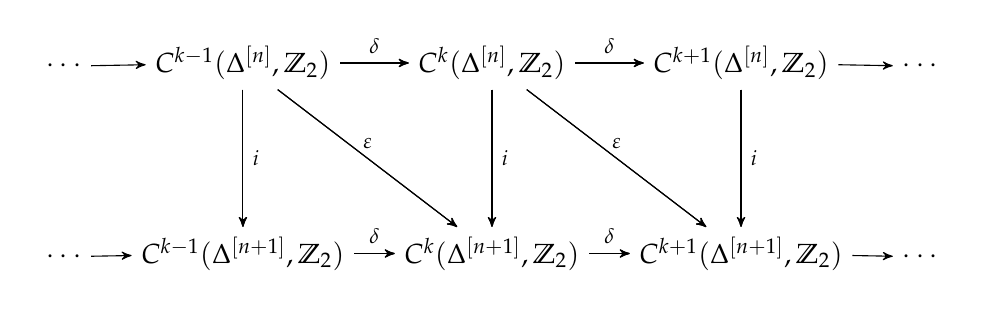
\begin{tikzpicture}
  \matrix (m) [matrix of math nodes, row sep=5em, column sep=1.5em]
    { \cdots & C^{k-1}(\Delta^{[n]},\mathbb{Z}_2) & C^{k}(\Delta^{[n]},\mathbb{Z}_2) & C^{k+1}(\Delta^{[n]},\mathbb{Z}_2) & \cdots \\
      \cdots & C^{k-1}(\Delta^{[n+1]},\mathbb{Z}_2) & C^{k}(\Delta^{[n+1]},\mathbb{Z}_2) & C^{k+1}(\Delta^{[n+1]},\mathbb{Z}_2) & \cdots \\ };
  { [start chain] \chainin (m-1-1);
    \chainin (m-1-2);
    { [start branch=A] \chainin (m-2-2)
        [join={node[right,labeled] {i}}];}
    \chainin (m-1-3) [join={node[above,labeled] {\delta}}];
    { [start branch=B] \chainin (m-2-3)
        [join={node[right,labeled] {i}}];}
    \chainin (m-1-4) [join={node[above,labeled] {\delta}}];
    { [start branch=C] \chainin (m-2-4)
        [join={node[right,labeled] {i}}];}
    \chainin (m-1-5); }
  { [start chain] \chainin (m-2-1);
    \chainin (m-2-2);
    \chainin (m-2-3) [join={node[above,labeled] {\delta}}];
    \chainin (m-2-4) [join={node[above,labeled] {\delta}}];
    \chainin (m-2-5); }
  { [start chain] \chainin (m-1-2);
  	\chainin (m-2-3) [join={node[above,labeled] {\varepsilon}}]; }
  { [start chain] \chainin (m-1-3);
  	\chainin (m-2-4) [join={node[above,labeled] {\varepsilon}}]; }
\end{tikzpicture}
 \caption{Cochain complexes with coning maps}
 \label{figure3:Figure 3}
\end{figure}


Here \(i\) is induced by the natural inclusion \(\Delta^{[n]}\rightarrow\Delta^{[n+1]}\) and the coning map can be again translated from the combinatorial version by \(\varepsilon(c)=supp^{-1}(\varepsilon(supp(c)))\). Another equivalent way to define the coning map algebraically is by \(\varepsilon=\delta i+i\delta\). Note, that the maps \(i\) and \(\varepsilon\) are both norm preserving.

\begin{lem}\label{lemma9}
According to the maps defined above, we have the following relations:
\begin{enumerate}
\item \(supp(i\delta(c))\subseteq supp(\delta i(c))\), for any cochain \(c\)
\item \(\delta\varepsilon=\varepsilon\delta\)
\item \(\delta\varepsilon=\delta i\delta\)
\item \(\|\varepsilon(c)\|=\|\delta i(c)\|-\|i\delta(c)\|\), for any cochain \(c\)
\end{enumerate}
\begin{proof}
(1) The support of \(i\delta(c)\) consists of all simplices from \(\Delta^{[n]}\) (in the appropriate dimension), which contain an odd number of simplices from \(supp(c)\) as a face. These are clearly contained in the set of simplices from \(\Delta^{[n+1]}\), which contain an odd number of simplices from \(supp(c)\) as a face.\\
(2) \(\delta\varepsilon=\delta(\delta i + i\delta)=\delta\delta i + \delta i \delta=\delta i\delta=i\delta\delta + \delta i\delta=(i\delta + \delta i)\delta = \varepsilon\delta\).\\
(3) Is already contained in the proof of (2).\\
(4) Follows immediately from (1).
\end{proof}
\end{lem}

\begin{prop}\label{proposition9}
Let \(c\in C^k(\Delta^{[n]},\mathbb{Z}_2)\) not be a cosystole, then \(\varepsilon(c)\) is not a cosystole.
\begin{proof}
Let \(c\in C^k(\Delta^{[n]},\mathbb{Z}_2)\) not be a cosystole. Then there exists a cochain \(d'\in C^{k-1}(\Delta^{[n]},\mathbb{Z}_2)\), such that \(\|\delta(d')+c\| < \|c\|\) and so, defining \(d:=\varepsilon(d')\) and using Lemma \ref{lemma9} (2) we get:
\begin{align}
\|\delta(d)+\varepsilon(c)\|&=\|\delta(\varepsilon(d'))+\varepsilon(c)\|\notag\\
&=\|\varepsilon(\delta(d')+c)\|\notag\\
&=\|\delta(d')+c\|\notag\\
&<\|c\|=\|\varepsilon(c)\|\notag
\end{align}
\end{proof}
\end{prop}
We conjecture that the reverse is also true and we can already prove a weaker statement. Before, consider the following small but important observation.\\
Note, that any cochain \(d\in C^k(\Delta^{[n+1]},\mathbb{Z}_2)\) can uniquely be represented as\\
\(d=\varepsilon(d_1)+i(d_2)\), with \(d_1\in C^{k-1}(\Delta^{[n]},\mathbb{Z}_2)\) and \(d_2\in C^k(\Delta^{[n]},\mathbb{Z}_2)\). Regarding the proof of Proposition \ref{proposition9}, we see that if we write \(d=\varepsilon(d')\) as \(\varepsilon(d_1)+i(d_2)\), the second part \(i(d_2)\) vanishes, espacially we have \(\delta(d_2)=0\). The following statement shows, that if we could always construct a \(d=\varepsilon(d_1)+i(d_2)\) satisfying \(\|\delta(d)+\varepsilon(c)\|<\|\varepsilon(c)\|\) and \(\delta(d_2)=0\), then the reverse of the preceding Proposition would be true as well.
\begin{prop}\label{proposition10}
Let \(\varepsilon(c)\in C^{k+1}(\Delta^{[n+1]},\mathbb{Z}_2)\) not be a cosystole. If there exists a cochain \(d=\varepsilon(d_1)+i(d_2)\in C^k(\Delta^{[n+1]},\mathbb{Z}_2)\), such that \(\|\delta(d)+\varepsilon(c)\|<\|\varepsilon(c)\|\) and \(\delta(d_2)=0\), then \(c\) is not a cosystole.
\begin{proof}
Let \(d=\varepsilon(d_1)+i(d_2)\in C^k(\Delta^{[n+1]},\mathbb{Z}_2)\) satisfy the assumptions. Then there exists a \(d_2'\in  C^{k-1}(\Delta^{[n]},\mathbb{Z}_2)\), such that \(d_2=\delta(d_2')\). This is because \(\Delta^{[n]}\) is contractible, so cohomology vanishes and kernel and image of \(\delta\) coinside. Now we have:
\begin{align}
\|\delta(d_1+d_2')+c\|&=\|\delta(d_1)+d_2+c\|\notag\\
&=\|\varepsilon(\delta(d_1)+d_2+c)\|\notag\\
&=\|\delta\varepsilon(d_1)+\varepsilon(d_2)+\varepsilon(c)\|\notag\\
&=\|\delta\varepsilon(d_1)+\delta i(d_2)+\varepsilon(c)\|\notag\\
&=\|\delta(\varepsilon(d_1)+i(d_2))+\varepsilon(c)\|\notag\\
&<\|\varepsilon(c)\|=\|c\|\notag
\end{align}
Hence, \(c\) is not a cosystole.
\end{proof}
\end{prop}
Now we have to deal with the following challenge. If we have some cochain \(d=\varepsilon(d_1)+i(d_2)\), satisfying \(\|\delta(d)+\varepsilon(c)\|<\|\varepsilon(c)\|\), but unfortunately not satisfying \(\delta(d_2)=0\), we have to find a better "substitude" for \(d\), which does the same job, meaning we have to find a \(d'=\varepsilon(d_1')+i(d_2')\), satisfying \(\|\delta(d')+\varepsilon(c)\|<\|\varepsilon(c)\|\) and \(\delta(d_2')=0\), but until now this seems pretty difficult to find.\\
The central problem which makes it difficult to deal with cosystoles in general is, that compared with cut-minimal graphs we have almost no handy tools beside the original definition yet to show cosystolicity of a given cochain. 
% Chapter 3

\chapter{Cut-minimal graphs and Cheeger graphs of a simplex}

\label{Chapter3}

In this chapter we start from the work of Kozlov (see \cite{1}) in which a graph theoretical approach to the first Cheeger constant of a simplex was developed. In the course of this approach the so called cut-minimal graphs appeared, which exactly describe \(1\)-cosystoles in a very intuitive way. As a consequence of the first main result of this chapter (Theorem \ref{theorem1}) we will determinine the dimension and partly the homology of the simplicial complex \(\mathcal{C}_1(\Delta^{[n]})\). In the second part of this chapter, we face the research on the first Cheeger constant of a simplex by investigating combinatorial properties of the Cheeger graphs which are just the graphic version of the \(1\)-Cheeger cosystoles.

\section{Basic definitions and properties of cut-minimal graphs}
The following definition and some words about motivation and intuition for it can be found in \cite{1} (Definition 2.3).

\begin{defi}
Consider a graph \(G=([n],E)\). For any subsets \(A,B\subset [n]\) define
\[
E_G(A,B)\coloneqq \{(v,w)\in E\: :\: v\in A\text{, }w\in B\}
\]
and
\[
NE_G(A,B)\coloneqq \{(v,w)\notin E\: :\: v\in A\text{, }w\in B\}
\]
A graph \(G=([n],E)\) is called \textbf{cut-minimal}, if for every \(S\subset[n]\) we have
\[
|E_G(S,[n]\setminus S)|\leq |NE_G(S,[n]\setminus S)|,
\]
which is equivalent to
\[
|E_G(S,[n]\setminus S)|\leq\frac{|S|(n-|S|)}{2}
\]
\end{defi}

Note, that there is a one-to-one correspondence between the graphs on \(n\) vertices and the \(1\)-chains  as follows:\\
For a graph \(G=([n],E)\) set \(c_G\coloneqq \sum\limits_{e\in E}e\in C_1(\Delta^{[n]})\) and for a chain \(c\in C_1(\Delta^{[n]})\) set \(G_c\coloneqq ([n],E)\), with \(E\coloneqq \supp(c)\). Considering characteristic cochains we also get a one-to-one corresponsing between graphs on \(n\) vertices and \(1\)-cochains and it is easy to see that a graph \(G=([n],E)\) is cut-minimal if and only if the corresponding cochain \(c_G^*\) is a cosystole.

\begin{rem}\label{remark1}
In fact for a graph \(G\) to be cut-minimal we only need to require the preceding condition holding for all \(S\subset [n]\), such that \(1\leq|S|\leq\frac{n}{2}\), since for all \(S\subset [n]\) we have \(E_G(S,[n]\setminus S)=E_G([n]\setminus S,S)\) and \(NE_G(S,[n]\setminus S)=NE_G([n]\setminus S,S)\).
\end{rem}

\begin{expl}
A simple cycle respresented by the graph \(G=([n],E)\) with\\
\(E\coloneqq \{(i,i+1)\: :\: 1\leq i\leq n-1\}\cup\{(n,1)\}\) is cut-minimal for all \(n\geq 7\) as follows. One can easily see that for all \(S\subset [n]\), such that \(|S|\leq\frac{n}{2}\), we have \(|E_G(S,[n]\setminus S)|\leq 2|S|\) and the inequality \(2|S|\leq\frac{|S|(n-|S|)}{2}\) holds for all \(n\geq |S|+4\), so by \(|S|\leq\frac{n}{2}\) the statement is true for all \(n\geq 7\).
\end{expl}

\begin{defi}
For any \(n\geq 1\) we define the set of all cut-minimal graphs on \(n\) vertices:
\[
CMG(n)\coloneqq \{G=([n],E)\: :\: G\text{ is cut-minimal}\}
\]
\end{defi}

\section{Maximal cut-minimal graphs}

Let us study the the topological and simplicial structure of the simplicial complex \(\mathcal{C}_1(\Delta^{[n]})\) which was, more generally, already introduced in the preceding chapter. Understanding this complex will help us to explore combinatorial properties of the cut-minimal graphs on a certain number of vertices.\\
The first thing we will do is to determine the maximum number of edges, a cut-minimal graph on a certain number of vertices can have, which immediately gives us the dimension of \(\mathcal{C}_1(\Delta^{[n]})\).

\begin{prop}\label{proposition3}
\(C_{max}(\Delta^{[n]},1)\geq\binom{\left\lceil\frac{n}{2}\right\rceil}{2}+\binom{\left\lfloor\frac{n}{2}\right\rfloor}{2}\)
\begin{proof}
Let us construct a graph \(G\) on \(n\) vertices as follows. Choose a set \(V'\subset [n]\), such that \(|V'|=\left\lceil\frac{n}{2}\right\rceil\) and connect each pair of vertices from \(V'\) by an edge. Then connect each pair of the remaining \(\left\lfloor\frac{n}{2}\right\rfloor\) vertices by an edge. In other words our graph consists of two complete graphs. If \(n\) is even, they are identical, otherwise they differ by one vertex. In total we get \(\binom{\left\lceil\frac{n}{2}\right\rceil}{2}+\binom{\left\lfloor\frac{n}{2}\right\rfloor}{2}\) edges. We will show that this graph is cut-minimal.\\
Let \(S\subset [n]\) and define \(A\coloneqq S\cap V'\) and \(B\coloneqq S\setminus A\). If \(n\) is even, we have:
\begin{align}
|E_G(S,[n]\setminus S)|&=|A|(\frac{n}{2}-|A|)+|B|(\frac{n}{2}-|B|)\notag\\
&=\frac{n|A|}{2}-|A|^2+\frac{n|B|}{2}-|B|^2\notag\\
&=\frac{n|S|}{2}-(|A|^2+|B|^2)\notag
\end{align}
\begin{align}
&\leq\frac{n|S|}{2}-\frac{|S|^2}{2}\notag\\
&=\frac{|S|(n-|S|)}{2},\notag
\end{align}
where the inequality comes from:
\begin{align}
&\quad\quad\quad\:\, (|A|-|B|)^2\geq 0\notag\\
&\Longleftrightarrow\quad |A|^2-2|A||B|+|B|^2\geq 0\notag\\
&\Longleftrightarrow\quad \frac{|A|^2}{2}-|A||B|+\frac{|B|^2}{2}\geq 0\notag\\
&\Longleftrightarrow\quad |A|^2+|B|^2\geq\frac{|A|^2}{2}+|A||B|+\frac{|B|^2}{2}\notag\\
&\Longleftrightarrow\quad |A|^2+|B|^2\geq\frac{|S|^2}{2}.\notag
\end{align}
If \(n\) is odd, we have:
\begin{align}
|E_G(S,[n]\setminus S)|&=|A|(\frac{n+1}{2}-|A|)+|B|(\frac{n-1}{2}-|B|)\notag\\
&=\frac{n|A|}{2}+\frac{|A|}{2}-|A|^2+\frac{n|B|}{2}-\frac{|B|}{2}-|B|^2\notag\\
&=\frac{n|S|}{2}-(|A|^2+|B|^2-\frac{|A|-|B|}{2})\notag\\
&\leq\frac{n|S|}{2}-\frac{|S|^2}{2}\notag\\
&=\frac{|S|(n-|S|)}{2},\notag
\end{align}
where the inequality comes from:
\begin{align}
&\quad\quad\quad\:\, (|A|-|B|)^2-(|A|-|B|)\geq 0\notag\\
&\Longleftrightarrow\quad (|A|-|B|)^2-|A|+|B|\geq 0\notag\\
&\Longleftrightarrow\quad |A|^2+|B|^2-|A|+|B|\geq 2|A||B|\notag\\
&\Longleftrightarrow\quad \frac{|A|^2}{2}+\frac{|B|^2}{2}-\frac{|A|}{2}+\frac{|B|}{2}\geq |A||B|\notag\\
&\Longleftrightarrow\quad |A|^2+|B|^2-\frac{|A|}{2}+\frac{|B|}{2}\geq \frac{|A|^2}{2}+\frac{2|A||B|}{2}+\frac{|B|^2}{2}\notag\\
&\Longleftrightarrow\quad |A|^2+|B|^2-\frac{|A|-|B|}{2}\geq\frac{(|A|+|B|)^2}{2}\notag\\
&\Longleftrightarrow\quad |A|^2+|B|^2-\frac{|A|-|B|}{2}\geq\frac{|S|^2}{2}.\notag
\end{align}
Hence, the constructed graph is cut-minimal.
\end{proof}
\end{prop}

Note, that we already proved the equivalent statement as Proposition \ref{proposition112}, since a simple calculation immediately shows that \(\binom{\left\lceil\frac{n}{2}\right\rceil}{2}+\binom{\left\lfloor\frac{n}{2}\right\rfloor}{2}=\binom{n}{2}-\left\lfloor\frac{n^2}{4}\right\rfloor\). Eventhough, it seemed to be worth to state this alternative proof, as it gets along with pure combinatorics, without using any algebraic properties. Furthermore, it gives an exact description of the "shape" of such a large cut-minimal graph.

\begin{rem}\label{remark3}
For further proofs and calculations it might be helpful to keep mind that we have:
\begin{align}
&\binom{\left\lceil\frac{n}{2}\right\rceil}{2}+\binom{\left\lfloor\frac{n}{2}\right\rfloor}{2}=\frac{n^2-2n+1}{4},&\text{ for }n\text{ odd, and}\notag \\
&\binom{\left\lceil\frac{n}{2}\right\rceil}{2}+\binom{\left\lfloor\frac{n}{2}\right\rfloor}{2}=\frac{n^2-2n}{4},&\text{ for }n\text{ even.}\notag
\end{align}
\end{rem}

Now, we are able to state the main theorem of this section, saying that the preceding estimate is even an upper bound.

\begin{thm}\label{theorem1}
\(C_{max}(\Delta^{[n]},1)=\binom{\left\lceil\frac{n}{2}\right\rceil}{2}+\binom{\left\lfloor\frac{n}{2}\right\rfloor}{2}\)
\begin{proof}
In a cut-minimal graph the maximum degree of each vertex is \(\left\lfloor\frac{n-1}{2}\right\rfloor\), so if \(n\) is even, by Remark \ref{remark3} we have:
\[
C_{max}(\Delta^{[n]},1)\leq\frac{n\left\lfloor\frac{n-1}{2}\right\rfloor}{2}=\frac{n^2-2n}{4}=\binom{\left\lceil\frac{n}{2}\right\rceil}{2}+\binom{\left\lfloor\frac{n}{2}\right\rfloor}{2}
\]
If \(n\) is odd, the situation becomes more complicated. We only know that
\[
C_{max}(\Delta^{[n]},1)\leq\frac{n\left\lfloor\frac{n-1}{2}\right\rfloor}{2}=\frac{n^2-n}{4},
\]
but in this case unfortunately the right hand side is bigger than \(\binom{\left\lceil\frac{n}{2}\right\rceil}{2}+\binom{\left\lfloor\frac{n}{2}\right\rfloor}{2}\), so we have to find a smaller upper bound for \(C_{max}(\Delta^{[n]},1)\). The following investigation shows, that a graph with \(\frac{n^2-n}{4}\) edges can not be cut-minimal anymore, which will lead to the requested bound.\\
Consider a cut-minimal graph \(G=([n],E)\), and choose a vertex \(v\in [n]\), such that\\
\(\deg_G(v)=\frac{n-1}{2}\). If such a vertex does not exist, using Remark \ref{remark3} we have
\[
|E|\leq\frac{n(\frac{n-1}{2}-1)}{2}=\frac{n^2-3n}{4}<\frac{n^2-2n+1}{4}=\binom{\left\lceil\frac{n}{2}\right\rceil}{2}+\binom{\left\lfloor\frac{n}{2}\right\rfloor}{2}
\]
and we are done. Now there exist exactly \(\frac{n-1}{2}\) vertices \(v_1,\ldots,v_{\frac{n-1}{2}}\in [n]\), such that \((v,v_i)\notin E\) for all \(i=1,\ldots,\frac{n-1}{2}\). If we had \(\deg_G(v_i)=\frac{n-1}{2}\) for one of these vertices, we would get
\[
|E_G(\{v,v_i\},[n]\setminus\{v,v_i\})|=2\frac{n-1}{2}=n-1>n-2=\frac{2(n-2)}{2},
\]
so \(G\) would not be cut-minimal anymore. It follows that the degree of these \(\frac{n-1}{2}\) vertices has to be at least one lower than assumed, so the number of edges has to be at least \(\frac{n-1}{4}\) lower than assumed, which provides the new inequality:
\begin{align}
C_{max}(\Delta^{[n]},1)&\leq\frac{n^2-n}{4}-\frac{n-1}{4}\notag\\
&=\frac{n^2-2n+1}{4}\notag\\
&=\binom{\left\lceil\frac{n}{2}\right\rceil}{2}+\binom{\left\lfloor\frac{n}{2}\right\rfloor}{2}\notag
\end{align}
Hence, we have \(C_{max}(\Delta^{[n]},1)\leq\binom{\left\lceil\frac{n}{2}\right\rceil}{2}+\binom{\left\lfloor\frac{n}{2}\right\rfloor}{2}\) in general and by Proposition \ref{proposition3} we are done.
\end{proof}
\end{thm}

A formula for the dimension of \(\mathcal{C}_1(\Delta^{[n]})\) follows immediately from the preceding theorem.

\begin{cor}
\(\dim(\mathcal{C}_1(\Delta^{[n]})=\binom{\left\lceil\frac{n}{2}\right\rceil}{2}+\binom{\left\lfloor\frac{n}{2}\right\rfloor}{2}-1\)
\end{cor}

We have seen that the proof of Proposition \ref{proposition3} even contains a description of the shape of a cut-minimal graph with the maximum number of edges, which furthermore provides information about how a top dimensional simplex is embedded in \(\mathcal{C}_1(\Delta^{[n]})\). Now, the following theorem which was developed in \cite{10} does not only represent a first statement about the homology of \(\mathcal{C}_1(\Delta^{[n]})\) but even shows that the construction in the proof of Proposition \ref{proposition3} is the only possible shape of such graphs (top dimensional simplices respectively).

\begin{thm}\label{theorem3}
\(H_{\dim(\mathcal{C}_1(\Delta^{[n]})}(\mathcal{C}_1(\Delta^{[n]}))\cong 0\)
\begin{proof}
We will first show, that a top dimensional simplex in \(\mathcal{C}_1(\Delta^{[n]})\) can only be represented as a graph of the type we constructed in the proof of Proposition \ref{proposition3}.\\
Let \(n\) be even. If we set \(n=2t+2\), then by the number \(C_{max}(\Delta^{[n]},1)\) and cut-minimality, the graph \(G\) corresponding to a top dimensional simplex in \(\mathcal{C}_1(\Delta^{[n]})\) must be \(t\)-regular. Furthermore, for any three pairwise distinct vertices \(v,w,u\in [n]\) by cut-minimality we have
\[
E_G(\{v,w,u\},[n]\setminus\{v,w,u\})\leq\frac{3(2t-1)}{2}=3t-\frac{3}{2},
\]
so by \(t\)-regularity among any three vertices at least two of them must be adjacent. Now choose a vertex \(v\in [n]\) and set \(A\) to be the set consisting of all vertices, which are not adjacent to \(v\). Then we have \(|A|=t+1\) by \(t\)-regularity and by the preceding result any two vertices in \(A\) have to be adjacent. Thus, \(A\) provides a complete graph on \(t+1\) vertices, so by \(t\)-regularity \([n]\setminus A\) must also provide a complete graph on \(t+1\) vertices. Hence, every top dimensional simplex in \(\mathcal{C}_1(\Delta^{[n]})\) (for \(n\) even) corresponds to a graph of that shape.\\
Let now \(n\) be odd. If we set \(n=2t+3\), then by the number \(C_{max}(\Delta^{[n]},1)\) and cut-minimality there exist at least \(t+2\) vertices having degree \(t+1\). Let \(A\) denote the set of these vertices. For any \(v,w\in A\), such that \(v\neq w\) we have:
\[
E_G(\{v,w\},[n]\setminus\{v,w\})\leq\frac{2(2t+3-2)}{2}=2t+1<2t+2=\deg_G(v)+\deg_G(w),
\]
so all vertices in \(A\) are adjacent. By cut-minimality again we have \(|A|=t+2\), so \(A\) provides a complete graph on \(t+2\) vertices. The number of remaining edges \(\binom{t+1}{2}\) shows, that the remaining \(t+1\) vertices must also provide a complete graph, which is disjoint from the first one, because any other constellation would destroy cut-minimality. Thus, every top dimensional simplex in \(\mathcal{C}_1(\Delta^{[n]})\) corresponds to a graph of the requested type again.\\
Now we see that deleting an edge from such a graph (which is the same as deleting a vertex from a top dimensional simplex) produces a graph corresponding to a simplex which appears as a face of one top dimensional simplex, but can not be a face of another top dimensional simplex, since we can not construct a graph of the requested type by adding an edge at any other place than the place where we just deleted it. Thus, all top dimensional simplices are at most connected via simplices of codimension 2, which implies that \(\mathcal{C}_1(\Delta^{[n]})\) can be continiously retracted to a complex of codimension 1 and so homology in top dimension vanishes.
\end{proof}
\end{thm}

\begin{defi}
A cut-minimal graph \(G=([n],E)\) is called \textbf{maximal}, if for all\\
\(e\in NE_G([n],[n])\) the graph \(G^e\coloneqq ([n],E\cup\{e\})\) is not cut-minimal. We denote the set of all maximal cut-minimal graphs on \(n\) vertices by \(MAX(n)\).
\end{defi}
Since deleting in edge in a cut-minimal graph produces a cut-minimal graph again, it turnes out that we only have to determine all maximal cut-minimal graphs to find all cut-minimal graphs.
\begin{defi}
Two graphs \(G=([n],E)\) and \(G'=([n],E')\) are called \textbf{isomorphic}, if there exists a map \(f:[n]\rightarrow [n]\), such that \((i,j)\in E\) if and only if \((f(i),f(j))\in E'\).\\
For a graph \(G=([n],E)\) the \textbf{isomorphism class} of \(G\) is the set
\[
\left\{G'=([n],E'):G'\text{ and }G\text{ are isomorphic}\right\}
\]
\end{defi}

\begin{rem}
Note, that an isomorphism of graphs preserves most properties studied in this chapter, especially cut-minimality and the constant \(h(G)\), studied in the next section.
\end{rem}

Figure \ref{figure2:Figure 2} illustrates, how the isomorphism classes of cut-minimal graphs on \(6\) vertices are arranged, where the connecting lines represent the relations between the classes refering to the deletion or addition of edges. Note, that the choosen representatives in the figure do not always satisfy the property of being a deletion or an addition of the shown representative of a class below or above, but in this case there is always another representative in the class which does. We see that beside the class of maximal cut-minimal graphs constructed in the proof of Proposition \ref{proposition3}, we have three more classes of maximal cut-minimal graphs here.

\newpage

\begin{figure}[ht]
\centering
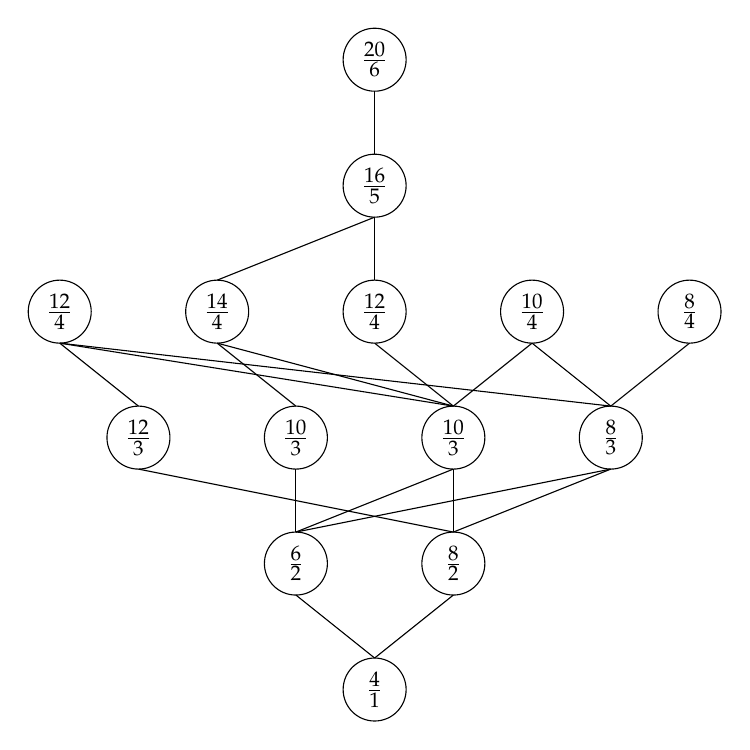
\begin{tikzpicture}
  [scale=.04,auto=left]
  
  \def\X{40}
  \def\Y{0}
  
  \def\x{\X -10}
  \def\y{\Y}
  
  \draw  (\x +10,\y +5) circle [radius=10cm] node {$\frac{4}{1}$};

  \def\x{\X -35}
  \def\y{\Y +40}
    
  \draw  (\x +10,\y +5) circle [radius=10cm] node {$\frac{6}{2}$};
  
  \draw  (\x +10,\y -5) -- (\x +35,\y -25);
  
  \def\x{\X +15}
  \def\y{\Y +40}
    
  \draw  (\x +10,\y +5) circle [radius=10cm] node {$\frac{8}{2}$};
  
  \draw  (\x +10,\y -5) -- (\x -15,\y -25);
  
  \def\x{\X -85}
  \def\y{\Y +80}
    
  \draw  (\x +10,\y +5) circle [radius=10cm] node {$\frac{12}{3}$};
  
  \draw  (\x +10,\y -5) -- (\x +110,\y -25);
  
  \def\x{\X -35}
  \def\y{\Y +80}
    
  \draw  (\x +10,\y +5) circle [radius=10cm] node {$\frac{10}{3}$};
  
  \draw  (\x +10,\y -5) -- (\x +10,\y -25);
  
  \def\x{\X +15}
  \def\y{\Y +80}
    
  \draw  (\x +10,\y +5) circle [radius=10cm] node {$\frac{10}{3}$};
  
  \draw  (\x +10,\y -5) -- (\x +10,\y -25);
  \draw  (\x +10,\y -5) -- (\x -40,\y -25);
  
  \def\x{\X +65}
  \def\y{\Y +80}
    
  \draw  (\x +10,\y +5) circle [radius=10cm] node {$\frac{8}{3}$};
  
  \draw  (\x +10,\y -5) -- (\x -40,\y -25);
  \draw  (\x +10,\y -5) -- (\x -90,\y -25);
  
  \def\x{\X -110}
  \def\y{\Y +120}
    
  \draw  (\x +10,\y +5) circle [radius=10cm] node {$\frac{12}{4}$};
  
  \draw  (\x +10,\y -5) -- (\x +35,\y -25);
  \draw  (\x +10,\y -5) -- (\x +135,\y -25);
  \draw  (\x +10,\y -5) -- (\x +185,\y -25);
  
  \def\x{\X -60}
  \def\y{\Y +120}
    
  \draw  (\x +10,\y +5) circle [radius=10cm] node {$\frac{14}{4}$};
  
  \draw  (\x +10,\y -5) -- (\x +35,\y -25);
  \draw  (\x +10,\y -5) -- (\x +85,\y -25);
  
  \def\x{\X -10}
  \def\y{\Y +120}
    
  \draw  (\x +10,\y +5) circle [radius=10cm] node {$\frac{12}{4}$};
  
  \draw  (\x +10,\y -5) -- (\x +35,\y -25);
  
  \def\x{\X +40}
  \def\y{\Y +120}
    
  \draw  (\x +10,\y +5) circle [radius=10cm] node {$\frac{10}{4}$};
  
  \draw  (\x +10,\y -5) -- (\x +35,\y -25);
  \draw  (\x +10,\y -5) -- (\x -15,\y -25);
  
  \def\x{\X +90}
  \def\y{\Y +120}
    
  \draw  (\x +10,\y +5) circle [radius=10cm] node {$\frac{8}{4}$};
  
  \draw  (\x +10,\y -5) -- (\x -15,\y -25);
  
  \def\x{\X -10}
  \def\y{\Y +160}
    
  \draw  (\x +10,\y +5) circle [radius=10cm] node {$\frac{16}{5}$};
  
  \draw  (\x +10,\y -5) -- (\x +10,\y -25);
  \draw  (\x +10,\y -5) -- (\x -40,\y -25);
  
  \def\x{\X -10}
  \def\y{\Y +200}
    
  \draw  (\x +10,\y +5) circle [radius=10cm] node {$\frac{20}{6}$};
  
  \draw  (\x +10,\y -5) -- (\x +10,\y -25);
\end{tikzpicture}
  \caption{The numbers \(h(G)\) for all cut-minimal graphs on 6 vertices}
  \label{figure2:Figure 3}
\end{figure}


Except for the maximal cut-minimal graphs with maximum number of edges we do not know anything about the remaining classes of cut-minimal graphs until now. The following statements now approach this challenge by providing new classes of cut-minimal graphs in general which do not appear as deletions of those largest maximal cut-minimal graphs.

\begin{lem}\label{lemma8}
Let \(u_1,\ldots,u_t,s_1,\ldots,s_t\in\mathbb{N}\cup\{0\}\), such that for all \(i=1,\ldots,t\) we have
\[
u_i+s_i\leq\sum_{\begin{subarray}{l}j=1\\ j\neq i\end{subarray}}^tu_j+s_j,
\]
then we have:
\[
\sum\limits_{i=1}^ts_i(u_i-\sum_{\begin{subarray}{l}j=1\\ j\neq i\end{subarray}}^tu_j)\leq 0
\]
\begin{proof}
If we have
\[
u_i\leq\sum_{\begin{subarray}{l}j=1\\ j\neq i\end{subarray}}^tu_j
\]
for all \(i=1,\ldots,t\), then we are done, since all \(u_i\)'s and \(s_i\)'s are positive. So, let there exist a \(k\in[t]\), such that
\[
u_k>\sum_{\begin{subarray}{l}j=1\\ j\neq k\end{subarray}}^tu_j
\]
Obviously, there is at most one unique \(u_k\) satisfying this property. Now for all \(i\neq k\) we have
\[
u_i-\sum_{\begin{subarray}{l}j=1\\ j\neq i\end{subarray}}^tu_j\leq -(u_k-\sum_{\begin{subarray}{l}j=1\\ j\neq k\end{subarray}}^tu_j),
\]
and furthermore we have
\[
s_k<\sum_{\begin{subarray}{l}j=1\\ j\neq k\end{subarray}}^ts_j
\]
by assumption and so we get:
\[
\sum_{\begin{subarray}{l}i=1\\ i\neq k\end{subarray}}^ts_i(u_i-\sum_{\begin{subarray}{l}j=1\\ j\neq i\end{subarray}}^tu_j)\leq-s_k(u_k-\sum_{\begin{subarray}{l}j=1\\ j\neq k\end{subarray}}^tu_j)
\]
Hence, we have:
\[
\sum\limits_{i=1}^ts_i(u_i-\sum_{\begin{subarray}{l}j=1\\ j\neq i\end{subarray}}^tu_j)\leq 0
\]
\end{proof}
\end{lem}

\begin{prop}
Let the largest connected component of a graph \(G=([n],E)\) not contain more than \(\frac{n}{2}\) vertices, then \(G\) is cut-minimal.
\begin{proof}
Let \(C_1,\ldots,C_t\subset [n]\) be the connected components of \(G\) and let \(S\subset [n]\), \(S_i\coloneqq S\cap C_i\) and \(U_i\coloneqq C_i\setminus S_i\) for all \(i=1,\ldots,t\). Then we have
\[
|E_G(S,[n]\setminus S)|\leq\sum\limits_{i=1}^t|S_i||U_i|
\] 
and
\[
|NE_G(S,[n]\setminus S)|\geq\sum\limits_{i=1}^t(|S_i|\sum_{\begin{subarray}{l}j=1\\ j\neq i\end{subarray}}^t|U_j|)
\]
So, we have to show that
\[
\sum\limits_{i=1}^t|S_i||U_i|\leq\sum\limits_{i=1}^t(|S_i|\sum_{\begin{subarray}{l}j=1\\ j\neq i\end{subarray}}^t|U_j|),
\]
which is equivalent to
\[
\sum\limits_{i=1}^t|S_i|(|U_i|-\sum_{\begin{subarray}{l}j=1\\ j\neq i\end{subarray}}^t|U_j|)\leq 0,
\]
but this follows directly from Lemma \ref{lemma8}, since by the assumption \(|C_i|\leq\frac{n}{2}\) for all \(i\), we have:
\[
|S_i|+|U_i|=|C_i|\leq\sum_{\begin{subarray}{l}j=1\\ j\neq i\end{subarray}}^t|C_j|=\sum_{\begin{subarray}{l}j=1\\ j\neq i\end{subarray}}^t|S_j|+|U_j|
\]
\end{proof}
\end{prop}

Let us now determine the counterpart of the number \(C_{max}(\Delta^{[n]},1)\), namely the minimal number of edges a non-cut-minimal graph can have, as it was already (more generally) defined in the preceding chapter.

\begin{thm}\label{theorem2}
\(C_{min}(\Delta^{[n]},1)=\left\lceil\frac{n}{2}\right\rceil\)
\begin{proof}
By Proposition \ref{proposition231} we get \(C_{min}(\Delta^{[n]},1)\leq\left\lceil\frac{n}{2}\right\rceil\). On the other hand if we have a graph \(G=([n],E)\) with \(|E|=\left\lceil\frac{n}{2}\right\rceil-1\), then it must be cut-minimal, since for any set of vertices \(S\subset[n]\), such that \(|S|<\frac{n}{2}\) we have \(\frac{|S|(n-|S|)}{2}\leq\frac{(|S|+1)(n-(|S|+1))}{2}\) and we have \(|E|=\left\lceil\frac{n}{2}\right\rceil-1=\left\lfloor\frac{n-1}{2}\right\rfloor\), so inductively \(|E(S,[n]\setminus S)|\leq\frac{|S|(n-|S|)}{2}\) holds for every \(S\subset [n]\) such that \(|S|\leq\frac{n}{2}\). Hence, we get \(C_{min}(\Delta^{[n]},1)\geq\left\lceil\frac{n}{2}\right\rceil\) and we are done.
\end{proof}
\end{thm}

Obviously, \(\mathcal{C}_1(\Delta^{[n]})\) contains all simplices of dimension lower than \(C_{min}(\Delta^{[n]},1)\), which leads to the following observation.

\begin{cor}
\(H_k(\mathcal{C}_1(\Delta^{[n]}))\cong 0\) for all \(1\leq k\leq\left\lceil\frac{n}{2}\right\rceil-3\)
\begin{proof}
By Theorem \ref{theorem2} \(\mathcal{C}_1(\Delta^{[n]})\) has a full \(k\)-skeleton for all \(k\leq\left\lceil\frac{n}{2}\right\rceil-2\) and we are done. 
\end{proof}
\end{cor}

Since adding a vertex to a cut-minimal graph will always preserve its property to be cut-minimal (see Lemma \ref{lemma132}), we can define the following natural embedding:

\begin{align}
i_n:CMG(n)&\longrightarrow CMG(n+1)\notag \\
([n],E)&\longmapsto ([n+1],E)\notag
\end{align}

Note, that the embedding \(i_n\) is just the graphic version of the more general embedding \(i_n^k\) for cochains from the preceding chapter, restricted to cut-minimal graphs.\\
Now, the first thing we see is that maximality of cut-minimal graphs always becomes destroyed by embedding them.

\begin{prop}
Let \(G\in MAX(n)\), then we have \(i_n(G)\notin MAX(n+1)\).
\begin{proof}
Let \(G=([n],E)\in MAX(n)\). If \(n\) is odd, Theorem \ref{theorem1} gives
\[
|E|\leq\frac{n^2-2n+1}{4}<\frac{n^2-n}{4}=\frac{n\frac{n-1}{2}}{2},
\]
so there exists a \(v\in [n]\), such that \(\deg_G(v)<\frac{n-1}{2}\). Now define\\
\(G'\coloneqq ([n+1],E\cup\{(v,n+1)\})\) and let \(S\subset [n+1]\), such that \(1\leq |S|\leq\frac{n+1}{2}\), then we have
\begin{align}
|E_{G'}(S,[n+1]\setminus S)|&\leq |E_G(S\setminus\{n+1\},[n]\setminus S)|+1\notag\\
&\leq\frac{|S|(n-|S|)}{2}+1\notag\\
&=\frac{|S|(n+\frac{2}{|S|}-|S|)}{2}\notag\\
&\leq\frac{|S|(n+1-|S|)}{2},\notag
\end{align}
for all \(S\subset [n+1]\), such that \(|S|\geq 2\). For \(|S|=1\), the upper condition is also satisfied, since we have \(\deg_G(v)<\frac{n-1}{2}\).\\
Hence, \(G'\) is cut-minimal and so we have \(i_n(G)=([n+1],E)\notin MAX(n+1)\).\\
If \(n\) is even, define \(G'\coloneqq ([n+1],E\cup (v,n+1))\) for an arbitrary \(v\in [n]\). Then by the same calculations as in the first part we have
\[
|E_{G'}(S,[n+1]\setminus S)|\leq\frac{|S|(n+1-|S|)}{2},
\]
for all \(S\subset [n+1]\) such that \(|S|\geq 2\), and for \(|S|=1\) we have:
\begin{align}
|E_{G'}(S,[n+1]\setminus S)|&\leq\text{max}\{\deg_{G'}(w):w\in[n+1]\}\notag\\
&\leq\left\lfloor\frac{n-1}{2}\right\rfloor +1\notag\\
&=\frac{n-2}{2}+1=\frac{n}{2}=\frac{(n+1)-1}{2}\notag
\end{align}
Hence, \(G'\) is cut-minimal and \(i_n(G)\notin MAX(n+1)\).
\end{proof}
\end{prop}

\section{Basic definitions and properties of Cheeger graphs}

The following definition is completely adopted from \cite{1} (Definition 2.6).
\begin{defi}\label{definition1}
Consider a graph \(G=([n],E)\), then we set:
\begin{small}
\[
T(G)\coloneqq \{(v,e)\: :\: v\in [n]\text{, }e=(w,u)\in E\text{, }v\notin e\text{, }|\{(v,w),(v,u),(w,u)\}\cap E\}|\text{ is odd}\}
\]
\end{small}
We have
\[
|T(G)|=\sum\limits_{e\in E}t(e),
\]
where for an edge \(e=(v,w)\in E\), we set
\[
t(e)\coloneqq \sum\limits_{\begin{subarray}{l}u\in[n]\\ u\neq v,w\end{subarray}}\tau_e(u),
\]
with
\begin{equation}
\tau_e(u)\coloneqq 
\begin{cases}
1,&\text{ if }(v,u),(w,u)\notin E\notag\\
\frac{1}{3},&\text{ if }(v,u),(w,u)\in E\notag\\
0,&\text{ otherwise}\notag
\end{cases}
\end{equation}
Furthermore, we define
\[
h(G)\coloneqq \frac{|T(G)|}{|E|},
\]
and call a cut-minimal graph \(G=([n],E)\) a \textbf{Cheeger graph}, if
\[
h(G)=\min\limits_{G'\in CMG(n)}h(G')
\]
The \textbf{first Cheeger constant of a simplex} is defined by
\[
h_1(\Delta^{[n]})\coloneqq h(G),
\]
where \(G\) is some Cheeger graph on \(n\) vertices.
\end{defi}
We already know by \cite{1} (Theorem 4.1 and Corollary 4.3) that we have \(\frac{n}{3}\leq h_1(\Delta{[n]})\leq\left\lceil\frac{n}{3}\right\rceil\) and the lower bound is archieved if \(n\) is not a power of \(2\). If two graphs \(G\) and \(G'\) belong to the same isomorphism class, we obviously have \(|T(G)|=|T(G')|\) and \(h(G)=h(G')\), so taking up the example from the preceding section, Figure \ref{figure3:Figure 3} shows the numbers \(h(G)\) for all cut-minimal graphs on \(6\) vertices with the same partially ordering as in Figure \ref{figure2:Figure 2} and we can see that there is one isomorphy class of Cheeger graphs attaining the Cheeger constant \(\frac{8}{4}\).

\begin{figure}[ht]
\centering
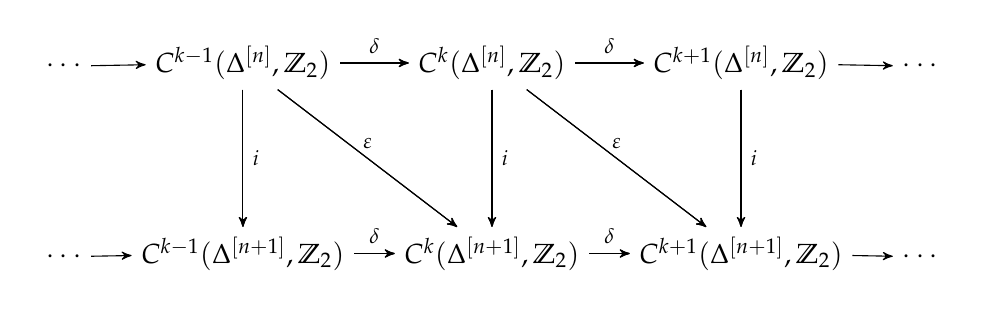
\begin{tikzpicture}
  \matrix (m) [matrix of math nodes, row sep=5em, column sep=1.5em]
    { \cdots & C^{k-1}(\Delta^{[n]},\mathbb{Z}_2) & C^{k}(\Delta^{[n]},\mathbb{Z}_2) & C^{k+1}(\Delta^{[n]},\mathbb{Z}_2) & \cdots \\
      \cdots & C^{k-1}(\Delta^{[n+1]},\mathbb{Z}_2) & C^{k}(\Delta^{[n+1]},\mathbb{Z}_2) & C^{k+1}(\Delta^{[n+1]},\mathbb{Z}_2) & \cdots \\ };
  { [start chain] \chainin (m-1-1);
    \chainin (m-1-2);
    { [start branch=A] \chainin (m-2-2)
        [join={node[right,labeled] {i}}];}
    \chainin (m-1-3) [join={node[above,labeled] {\delta}}];
    { [start branch=B] \chainin (m-2-3)
        [join={node[right,labeled] {i}}];}
    \chainin (m-1-4) [join={node[above,labeled] {\delta}}];
    { [start branch=C] \chainin (m-2-4)
        [join={node[right,labeled] {i}}];}
    \chainin (m-1-5); }
  { [start chain] \chainin (m-2-1);
    \chainin (m-2-2);
    \chainin (m-2-3) [join={node[above,labeled] {\delta}}];
    \chainin (m-2-4) [join={node[above,labeled] {\delta}}];
    \chainin (m-2-5); }
  { [start chain] \chainin (m-1-2);
  	\chainin (m-2-3) [join={node[above,labeled] {\varepsilon}}]; }
  { [start chain] \chainin (m-1-3);
  	\chainin (m-2-4) [join={node[above,labeled] {\varepsilon}}]; }
\end{tikzpicture}
 \caption{Cochain complexes with coning maps}
 \label{figure3:Figure 3}
\end{figure}


\section{A restriction on the size of connected components in\\ Cheeger graphs}
The following statement restricts the shape of Cheeger graphs in terms of the sizes of their connected components.

\begin{prop}
Let \(G=([n],E)\) be a Cheeger graph, then \(G\) must have a connected component of size at least \(n-\left\lceil\frac{n}{3}\right\rceil\).
\begin{proof}
Let \(C\subseteq [n]\) be the largest connected component of \(G\), then we obviously have
\[
\left\lceil\frac{n}{3}\right\rceil\geq h(G)\geq \frac{|E|(n-|C|)}{|E|}=n-|C|,
\]
which is equivalent to
\[
|C|\geq n-\left\lceil\frac{n}{3}\right\rceil
\]
\end{proof}
\end{prop}

A direct consequence of the preceding statement is, that for \(n\geq 6\) a Cheeger graph can never appear as a subgraph of a largest cut-minimal graph such as constructed in the proof of Proposition \ref{proposition3}.



\section{Embeddings of Cheeger graphs}

Based on the fact from the preceding chapter (see Lemma \ref{lemma132}) that adding a vertex to a cut-minimal graph will always result in a cut-minimal graph again, we will now study the consequences of adding a vertex to a Cheeger graph. It will turn out that the resulting graph will not be a Cheeger graph anymore. Using this fact we will be able to find a lower bound on the number of edges in Cheeger graphs. The following statement is just the graphic version of Proposition \ref{proposition113}.

\begin{prop}\label{proposition351}
Let \(G=([n],E)\) be a cut-minimal graph, then we have:
\[
h(i_n(G))=h(G)+1
\]
\end{prop}

\begin{prop}\label{proposition352}
Let \(G\in CMG(n)\), then \(i_n(G)\in CMG(n+1)\) is not a Cheeger graph.
\begin{proof}
Without loss of generality let \(G\) be a Cheeger graph. Otherwise, there exists a graph \(G'\in CMG(n)\), such that \(h(G')<h(G)\), so by Proposition \ref{proposition351} we get:
\[
h(i_n(G'))=h(G')+1<h(G)+1=h(i_n(G))
\]
Let now \(n+1\) not be a power of \(2\). Since we have \(h(G)\geq\frac{n}{3}\), by Proposition \ref{proposition351} we get
\[
h(i_n(G))\geq\frac{n}{3}+1=\frac{n+3}{3}>\frac{n+1}{3},
\]
so \(i_n(G)\) can not be a Cheeger graph. On the other hand if \(n+1\) is a power of \(2\), then \(n\) can not be a power of \(2\) and we have:
\[
h(i_n(G))=h(G)+1=\frac{n}{3}+1\geq\left\lceil\frac{n+1}{3}\right\rceil
\]
But by \cite{1} (Theorem 4.6) we have that \(h_1(\Delta^{[n+1]})<\left\lceil\frac{n+1}{3}\right\rceil\) holds if \(n+1\) is a power of \(2\), so \(i_n(G)\) can not be a Cheeger graph.
\end{proof}
\end{prop}

We can now calculate a lower bound for the number of edges in Cheeger graphs.

\begin{prop}
Let \(G=([n],E)\) be a Cheeger graph, then we have \(|E|\geq\left\lceil\frac{n-1}{2}\right\rceil\).
\begin{proof}
Assume we have \(|E|<\left\lceil\frac{n-1}{2}\right\rceil\). Then by Theorem \ref{theorem2} and since \(G\) must contain an isolated vertex, there exists a graph \(G'\in CMG(n-1)\) such that \(i_{n-1}(G')=G\), so by Proposition \ref{proposition352} \(G\) can not be a Cheeger graph and we are done.
\end{proof}
\end{prop}

\section{The case when n is a power of 2}

From \cite{1} (Corollary 4.3) we know that \(h(n)>\frac{n}{3}\) can only be valid, if \(n\) is a power of \(2\). An interesting question is, if this inequality is always strict for such \(n\). For a graph \(G=([n],E)\) and a vertex \(v\in [n]\) let us introduce the notation\\
\(A_v\coloneqq \{w\in [n]:(v,w)\in E\}\), so we have \(|A_v|=\deg_G(v)\). The following useful fact was given by Kozlov (see \cite{1}, Section 6.3).

\begin{lem}\label{lemma11:2}
Let \(G=([n],E)\) be a cut-minimal graph, then we have \(h(n)=\frac{n}{3}\) if and only if for each vertex \(v\in [n]\) we have \(|E(A_v\text{, }[n]\setminus A_v)|=|NE(A_v\text{, }[n]\setminus A_v)|\).
\end{lem}

We can now make a statement about the possible degrees a vertex in a Cheeger graph on \(n=2^t\) vertices can attain, assuming the first Cheeger constant exactly equals \(\frac{n}{3}\).

\begin{prop}\label{proposition321}
Let \(n=2^t\) and \(G=([n],E)\) be a cut-minimal graph, such that \(h(G)=\frac{n}{3}\). Then for each vertex \(v\in [n]\) we have \(|A_v|\in\left\{0\leq i\leq\frac{n-4}{2}:i\text{ is even }\right\}\setminus\{2\}\).
\begin{proof}
The proof of the fact, that \(|A_v|\) is even can be found in \cite{1} (Section 6.3). Since \(G\) is cut-minimal and \(n=2^t\), we have:
\[
|A_v|=|E(\{v\}\text{, }[n]\setminus\{v\})|\leq\left\lfloor\frac{n-1}{2}\right\rfloor=2^{t-1}-1
\]
But \(2^{t-1}-1\) is always odd, so we get:
\begin{equation}\label{equation2}
|A_v|\leq 2^{t-1}-2=\frac{n-4}{2}
\end{equation}
Now, assume there exists a \(v\in [n]\), such that \(|A_v|=2\), then by Lemma \ref{lemma11:2} we have
\[
|E(A_v\text{, }[n]\setminus A_v)|=|NE(A_v\text{, }[n]\setminus A_v)|=\frac{2(n-2)}{2}=n-2,
\]
so there must exist a \(w\in A_v\), such that \(|A_w|\geq\frac{n-2}{2}=\frac{2^t-2}{2}=2^{t-1}-1\), but this is a contradiction to \ref{equation2}.
\end{proof}
\end{prop}

\begin{expl}
In \cite{1} (Section 6.3) Kozlov already used the fact, that a vertex in a graph satisfying the conditions of the preceding proposition can not attain an odd degree to prove the strict bound \(h(8)>\frac{8}{3}\). Applying the preceding slightly stronger proposition we get this result immediately, since then every vertex in a Cheeger graph \(G=([8],E)\), satisfying \(h(G)=\frac{8}{3}\) must attain degree \(0\), which obviously leads to a contradiction.
\end{expl}

We can even say more about how the degrees of adjacent vertices interact in some cases as follows:

\begin{lem}
Let \(n=2^t\) and \(G=([n],E)\) be a cut-minimal graph, such that \(h(G)=\frac{n}{3}\). Then for each vertex \(v\in [n]\), such that \(|A_v|=4\) we have \(|A_w|=\frac{n-4}{2}\) for all \(w\in A_v\).
\begin{proof}
Let \(v\in [n]\) such that \(|A_v|=4\), then by Lemma \ref{lemma11:2} we have
\[
|E(A_v,[n]\setminus A_v)|=\frac{|A_v|(n-|A_v|)}{2}=2^{t+1}-8
\]
so there must exist a \(w\in A_v\) such that \(|A_w|\geq\frac{2^{t+1}-8}{4}=2^{t-1}-2\). Now, applying Proposition \ref{proposition321} we get that \(|A_w|=2^{t-1}-2=\frac{n-4}{2}\) holds for all \(w\in A_v\).

\end{proof}
\end{lem}
% Chapter 4

\chapter{Perspectives}

\label{Chapter4}

 

%----------------------------------------------------------------------------------------
%	THESIS CONTENT - APPENDICES
%----------------------------------------------------------------------------------------

\appendix % Cue to tell LaTeX that the following "chapters" are Appendices

% Include the appendices of the thesis as separate files from the Appendices folder
% Uncomment the lines as you write the Appendices

\chapter{Source code for the Cheeger Tool Box (CTB)}

\label{AppendixA}

The \textit{Cheeger Tool Box (CTB)} is a software library written in C++11, containing methods to handle some important tasks concerning the topic of Cheeger constants of a simplex, such as calculating the cosystolic norm and the coboundary expansion of a given cochain or calculating the \(k\)-th Cheeger constant of a simplex on \(n\) vertices. A cochain \(\varphi\in C^k(\Delta^{[n]})\) is always represented as a column vector with \(\binom{n}{k+1}\) (i.e. a matrix of one column and  \(\binom{n}{k+1}\) lines, such that every entry \(i\) is either \(1\) or \(0\), depending on if the \(i\)-th simplex in the uniform \(k\)-skeleton of \(\Delta^{[n]}\) is contained in the support of \(\varphi\). Here, the simplices of the uniform \(k\)-skeleton of \(\Delta^{[n]}\) are indexed lexicographically based on the contained vertices, which are indexed from \(1\) to \(n\).\\
To use the library, the reader should just save the single files in an ordering as shown in the labellings underneath each code block and include the header files into his own code. Note, that by now the methods only use the basic definitions of cosystolicity and Cheeger constants for the calculation. The interested reader is invited to use more results from theoretical research to improve its performance.\\

\lstinputlisting[language=C++]{CTB/headers/Matrix.h}

\lstinputlisting[language=C++]{CTB/sources/Matrix.cpp}

\lstinputlisting[language=C++]{CTB/headers/basics.h}

\lstinputlisting[language=C++]{CTB/sources/basics.cpp}

%----------------------------------------------------------------------------------------
%	BIBLIOGRAPHY
%----------------------------------------------------------------------------------------

%\printbibliography[heading=bibintoc]

%----------------------------------------------------------------------------------------
\begin{thebibliography}{1}
\bibitem{1}
Dmitry N. Kozlov, \textit{The first Cheeger constant of a simplex}, arXiv 1610:07136, 2016
\bibitem{2}
N. Linial, R. Meshulam, \textit{Homological connectivity of random 2-complexes}, Combinatorica 26, 2006,
no. 4, 475-487
\bibitem{3}
M. Gromov, \textit{Singularities, expanders and topology of maps. Part 2. From combinatorics to topology
via algebraic isoperimetry}, Geom. Funct. Anal. 20, (2010), no. 2, 416-526.
\bibitem{4}
M. Wallach, R. Meshulam, \textit{Homological connectivity of random k-dimensional complexes}, Random Structures Algorithms 34, 2009, no. 3, 408–417
\bibitem{5}
J. J. Sylvester and F. Franklin, \textit{A Constructive Theory of Partitions, Arranged in Three Acts, an Interact and an Exodion}, American Journal of Mathematics
Vol. 5, No. 1 (1882), pp. 251-330
\bibitem{6} Dmitry N, Kozlov, Roy Meshulam; \textit{Quantitative aspects of acyclicity}, 	arXiv:1802.03210 [math.CO], 2018
\bibitem{7} Peter Keevash; \textit{Hypergraph Tur\'{a}n problems},\\http://people.maths.ox.ac.uk/keevash/papers/turan-survey.pdf
\end{thebibliography}

\end{document}  
